\chapter{Diagramme de Gantt}\label{annexe-a}

\begin{figure}[htbp]
 \begin{center}
  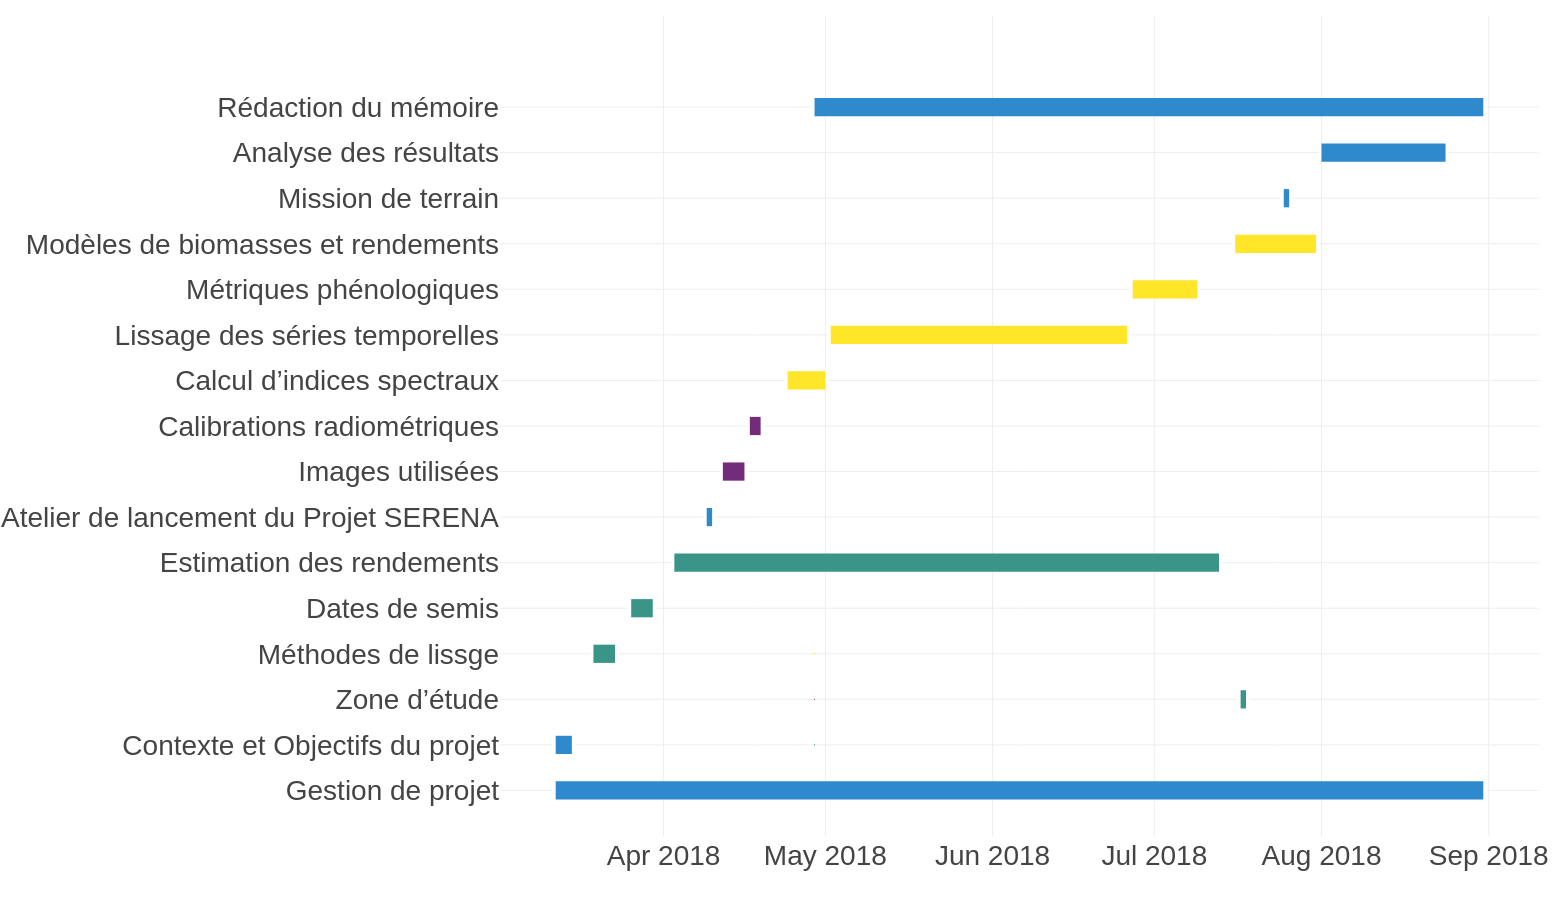
\includegraphics[scale=0.5]{annexes/gantt1.png} 
 \end{center}
\end{figure}

\begin{figure}[htbp]
 \begin{center}
  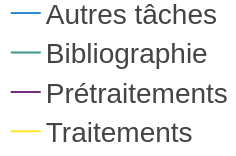
\includegraphics[scale=0.6]{annexes/gantt2.png} 
 \end{center}
\end{figure}


\chapter{Essais de lissage avec le filtre de Savitzky-Golay}\label{annexe-b}

Les figures ci-après représentent des essais de lissage avec le filtre de Savitzky-Golay sur quelques pixels appartenant aux parcelles suivies. Pour chaque pixel, nous faisons varier sur les colonnes le degré du polynôme d'ajustement et sur les lignes la largeur de la fenêtre de lissage, selon les valeurs proposées dans la littérature notamment par \citet{Chen2004}. 

\vspace{5mm}

\begin{figure}[htbp]
 \begin{center}
  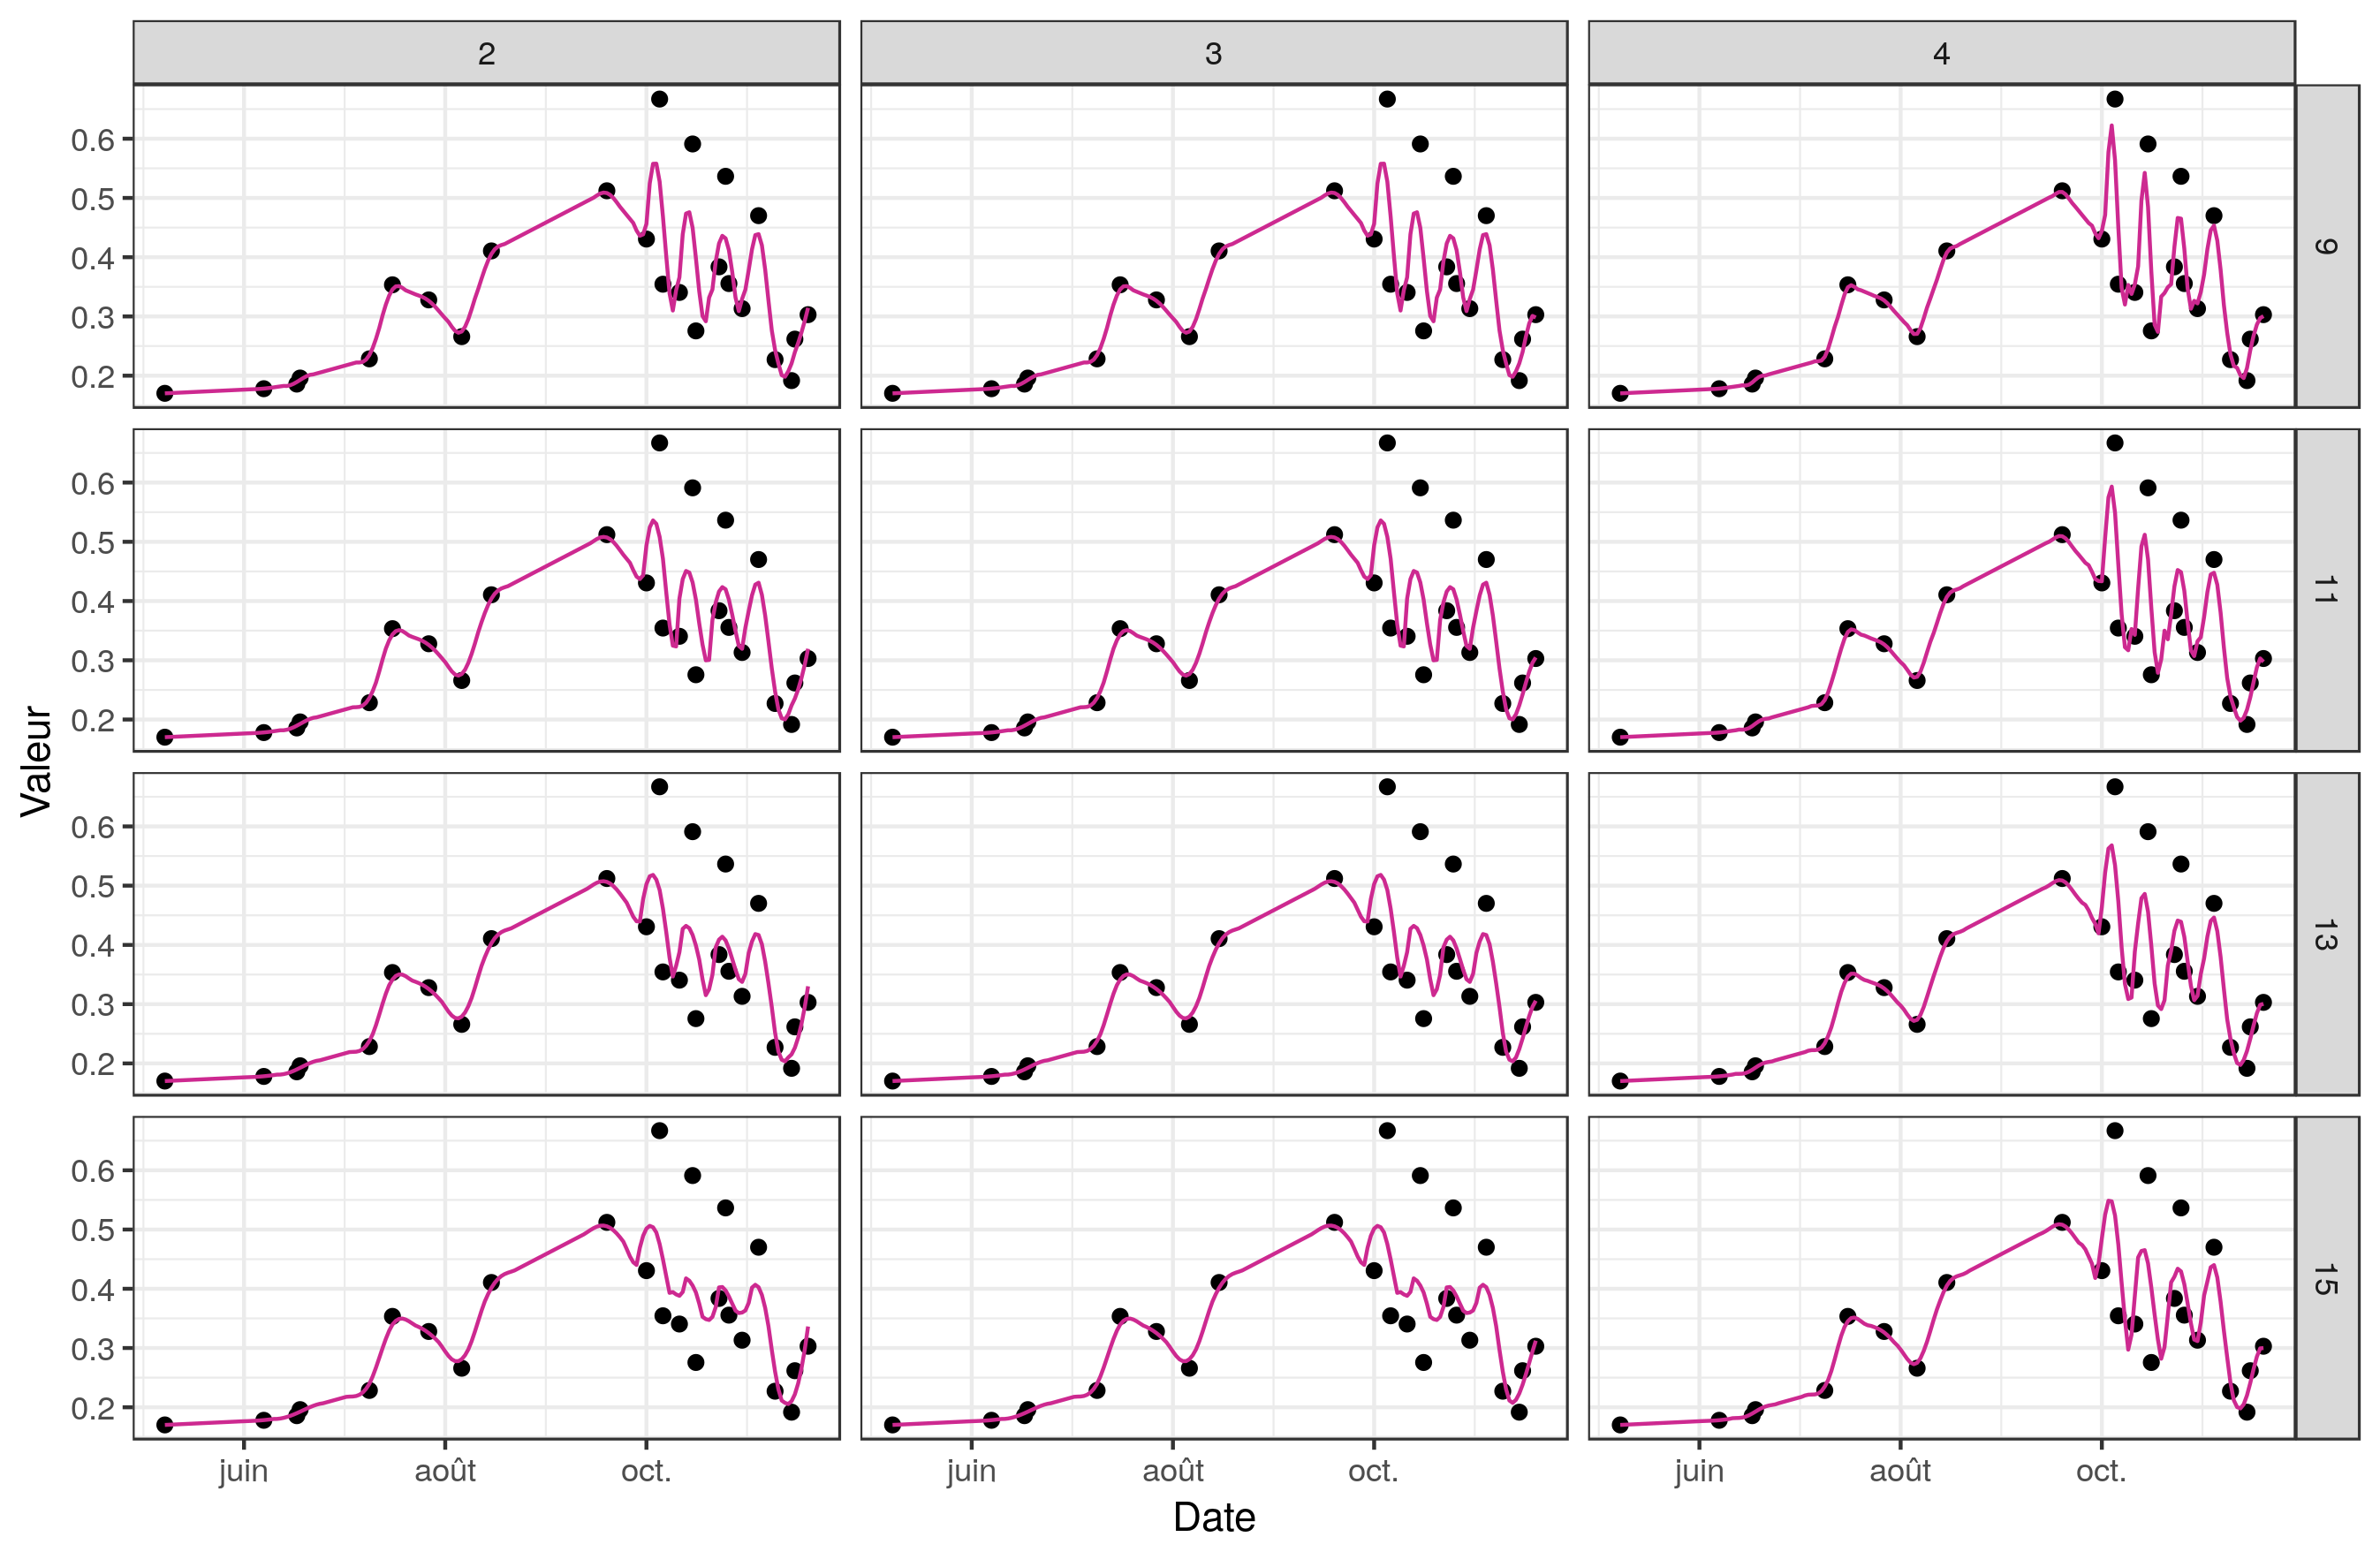
\includegraphics[scale=0.7]{annexes/savgol_prs_1.png} 
 \end{center}
 %\caption{Quelques résultats du lissage de la série temporelle rectifiée}
 %\label{fig-lissage-prscor}
\end{figure}

\begin{figure}[htbp]
 \begin{center}
  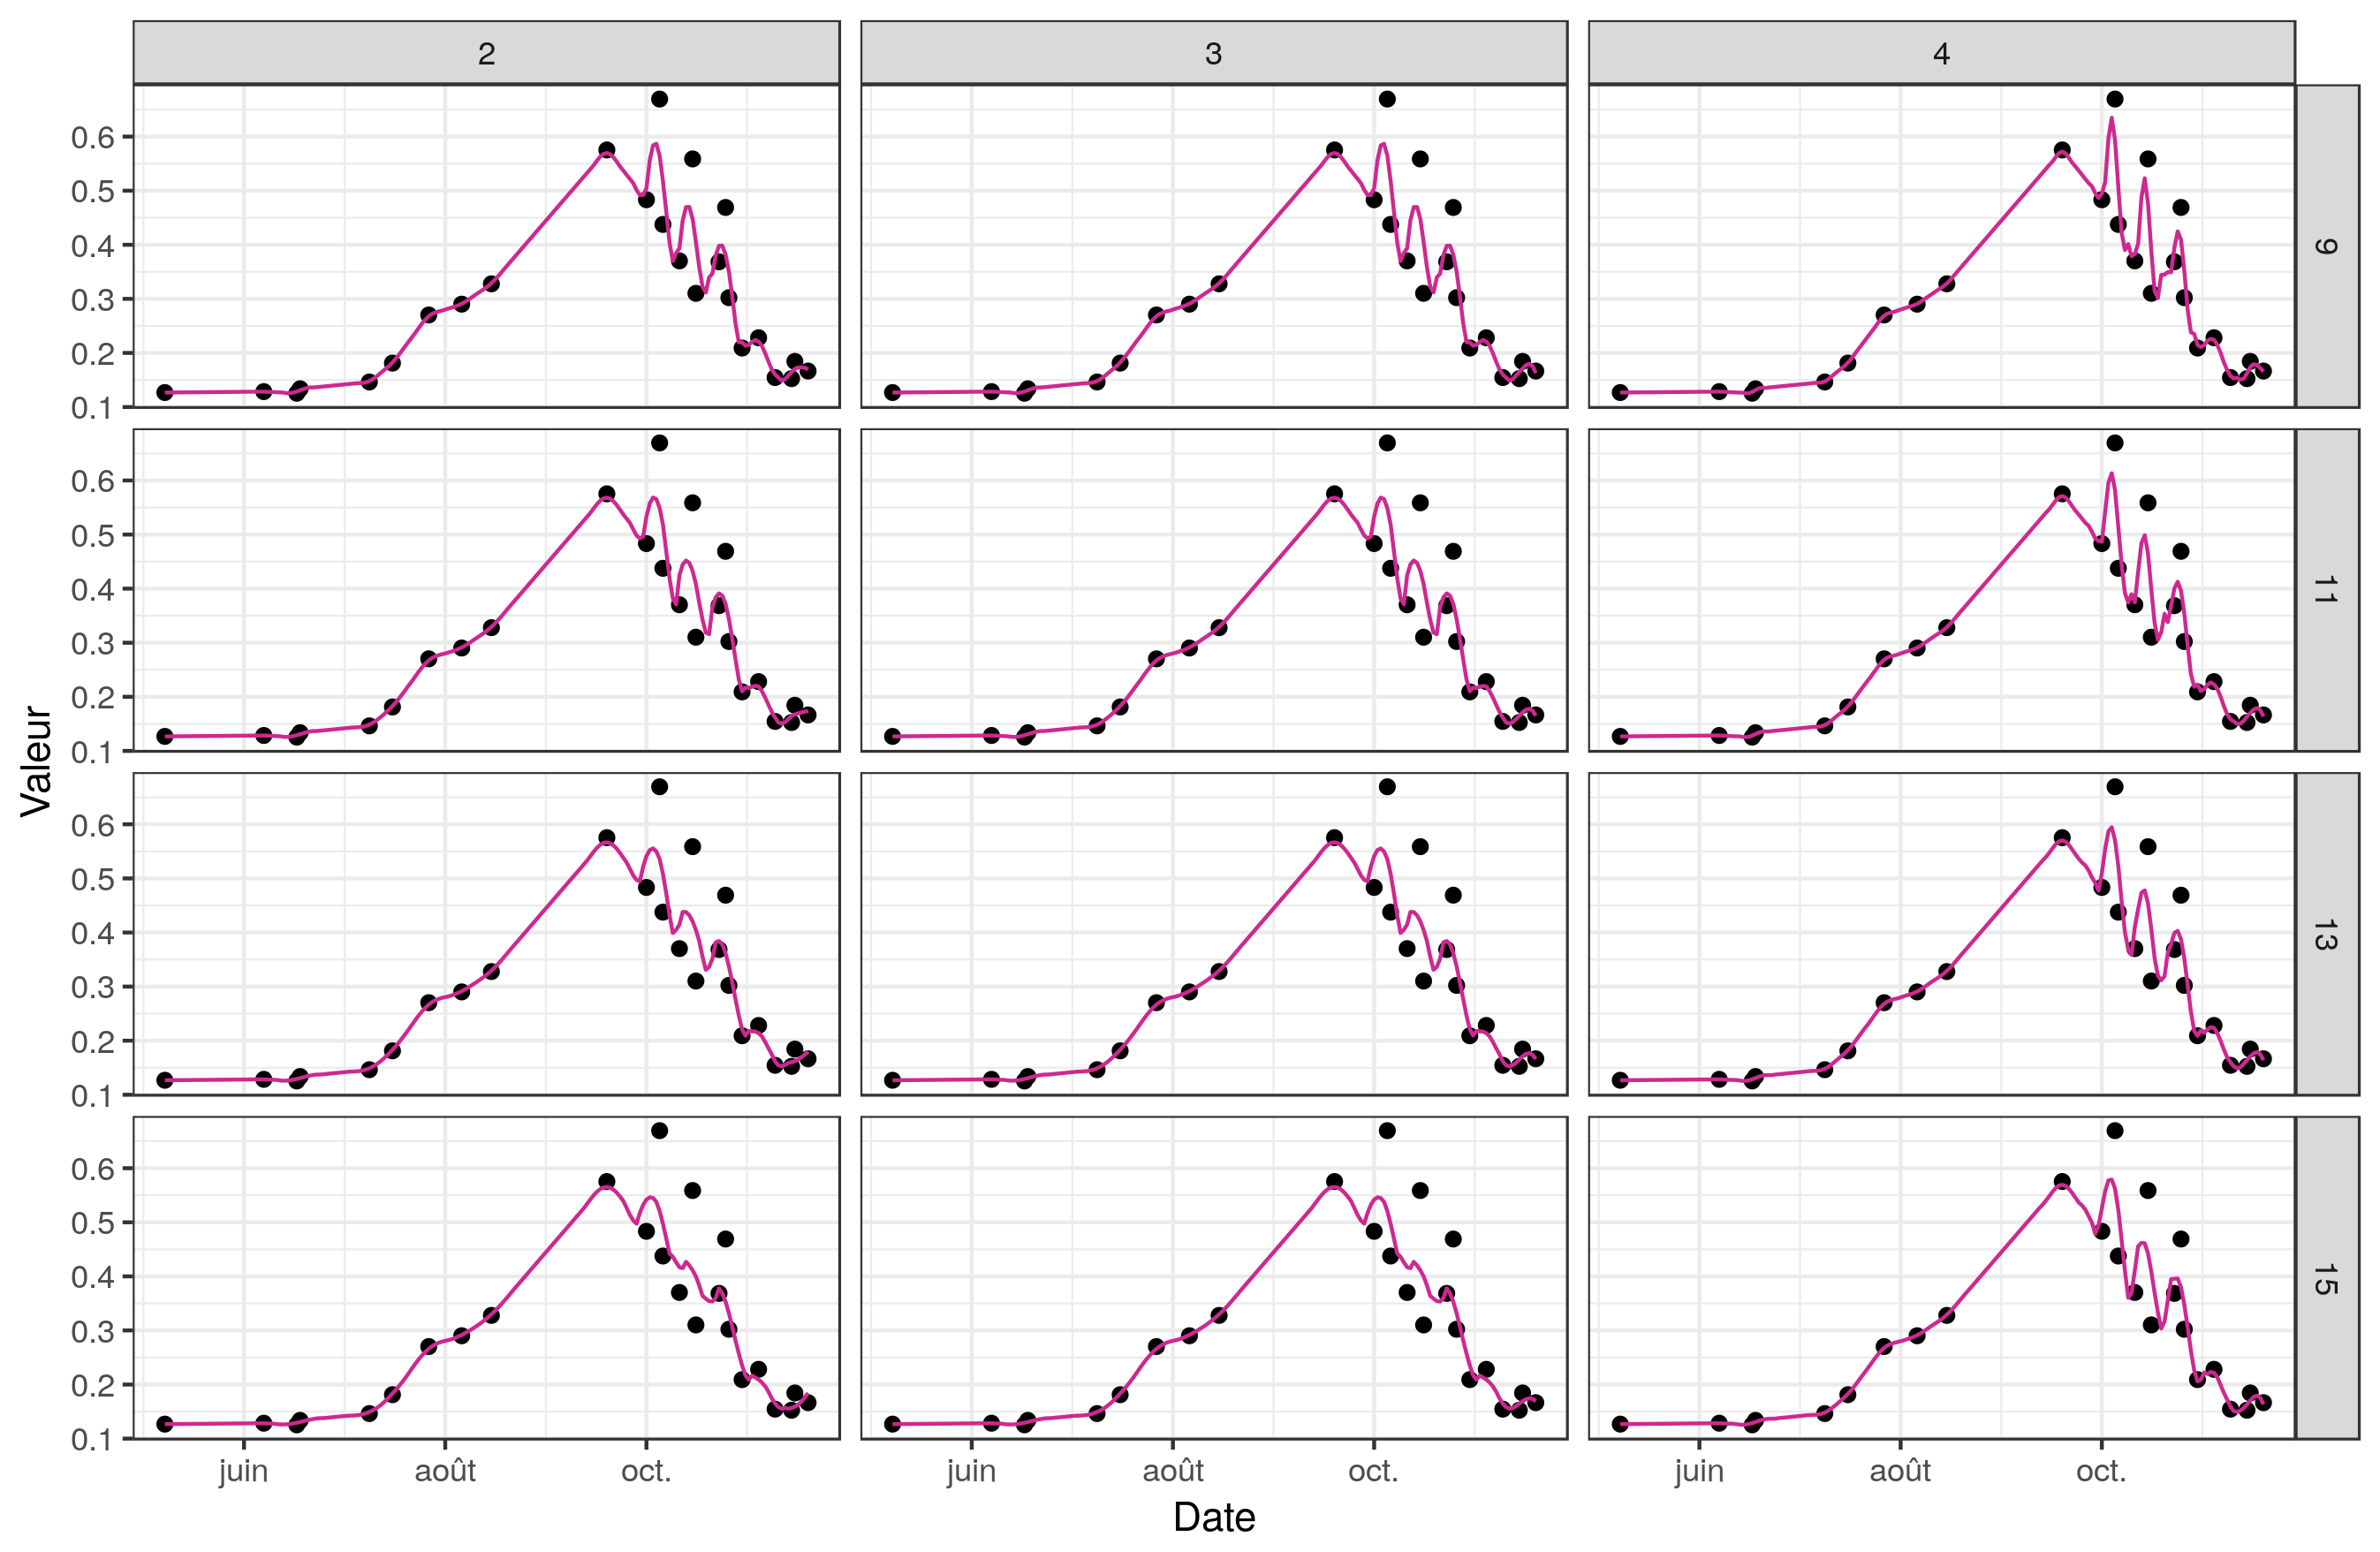
\includegraphics[scale=0.7]{annexes/savgol_prs_2.png} 
 \end{center}
 %\caption{Quelques résultats du lissage de la série temporelle rectifiée}
 %\label{fig-lissage-prscor}
\end{figure}

\begin{figure}[htbp]
 \begin{center}
  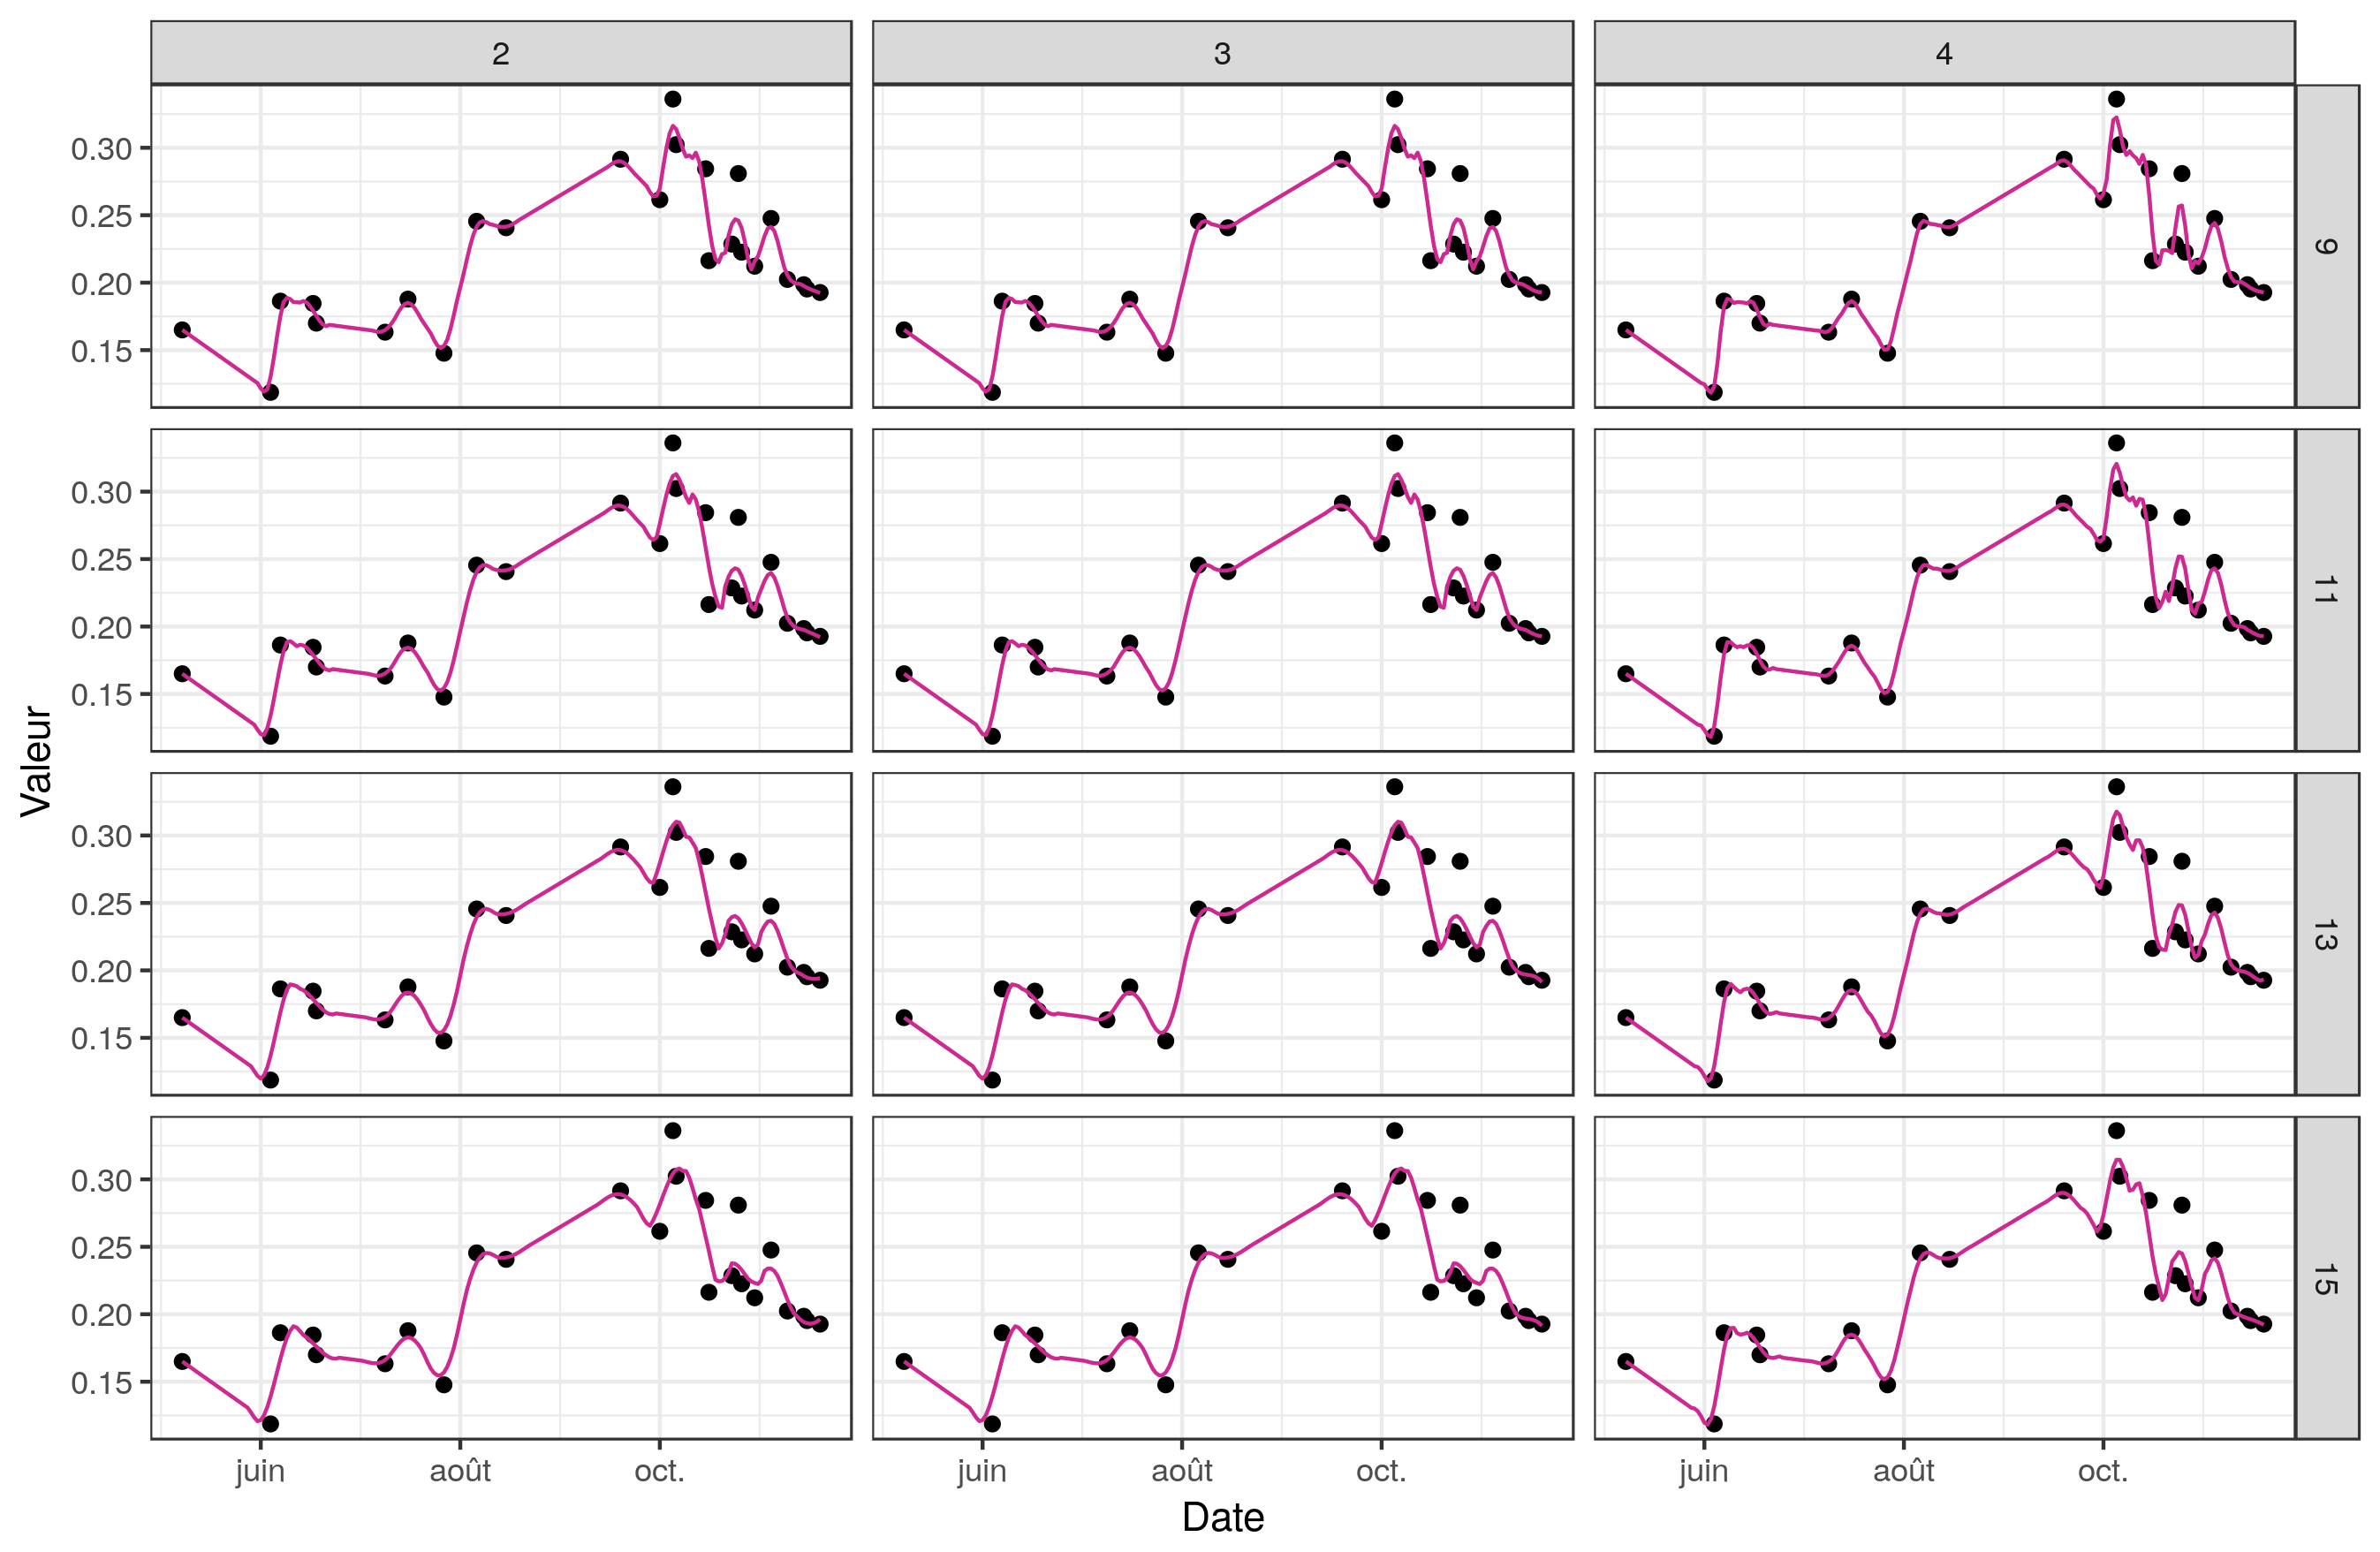
\includegraphics[scale=0.7]{annexes/savgol_prs_3.png} 
 \end{center}
 %\caption{Quelques résultats du lissage de la série temporelle rectifiée}
 %\label{fig-lissage-prscor}
\end{figure}

\chapter{Estimation des SOS et EOS sans le jeu ANR CERAO}\label{annexe-c}

\begin{figure}[htbp]
 \begin{center}
  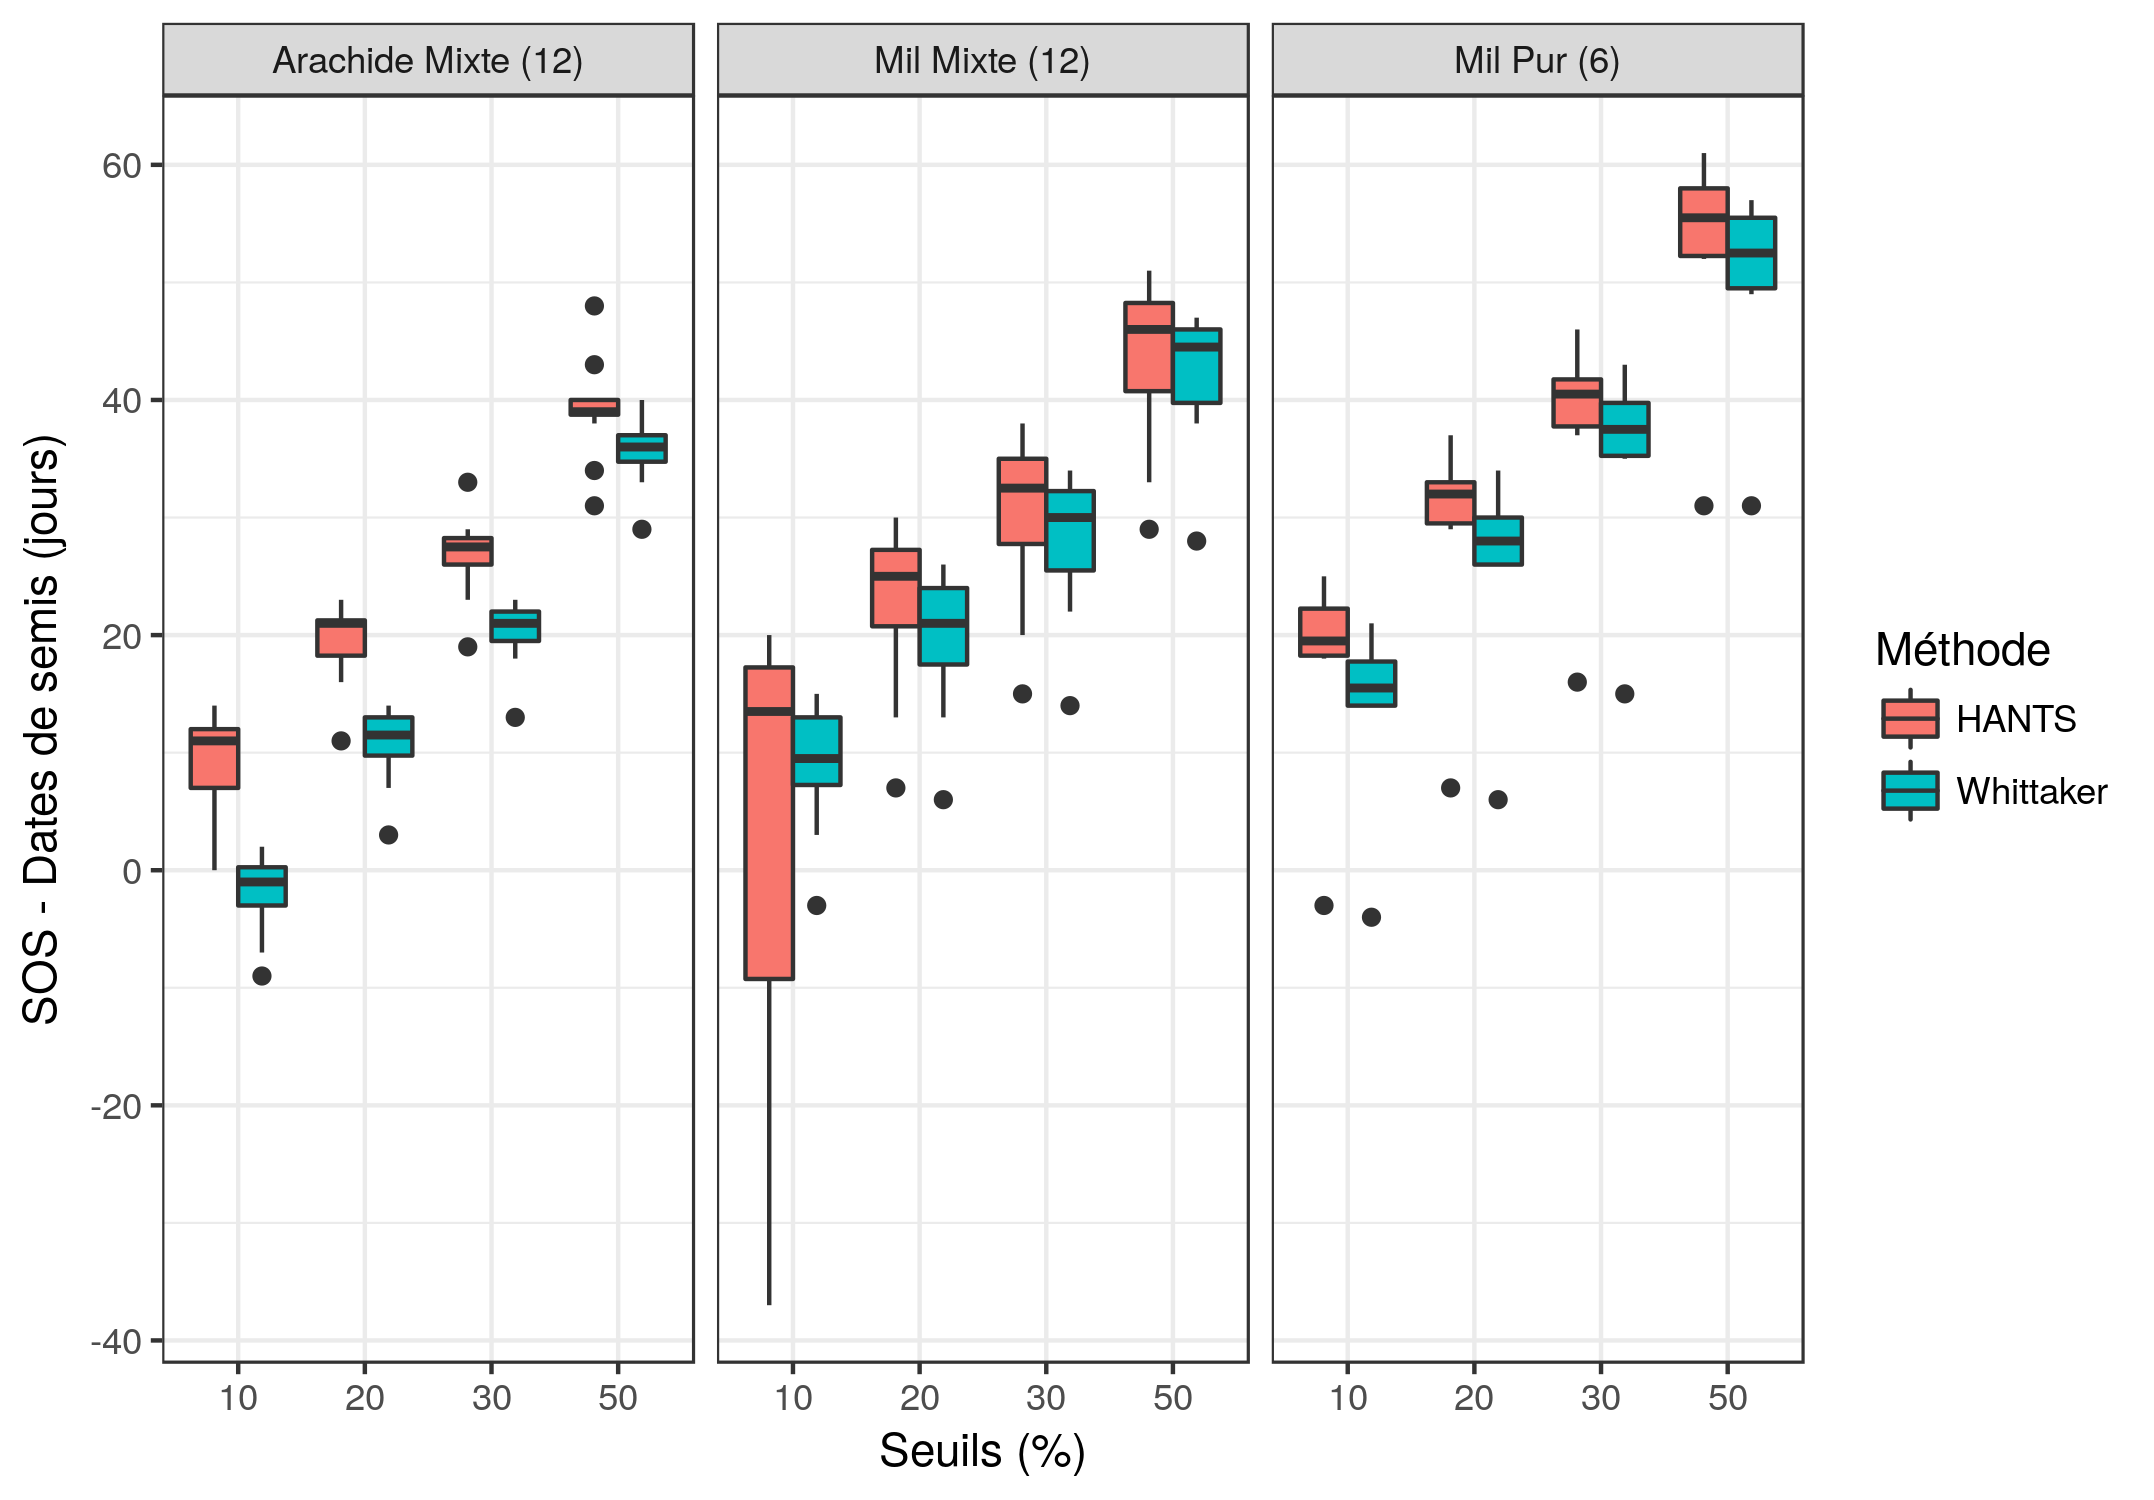
\includegraphics[scale=0.8]{annexes/SOS_Boxplot_Oracle.png} 
 \end{center}
 \caption*{Distribution des écarts entre SOS et dates de semis}
\end{figure}

\begin{figure}[htbp]
 \begin{center}
  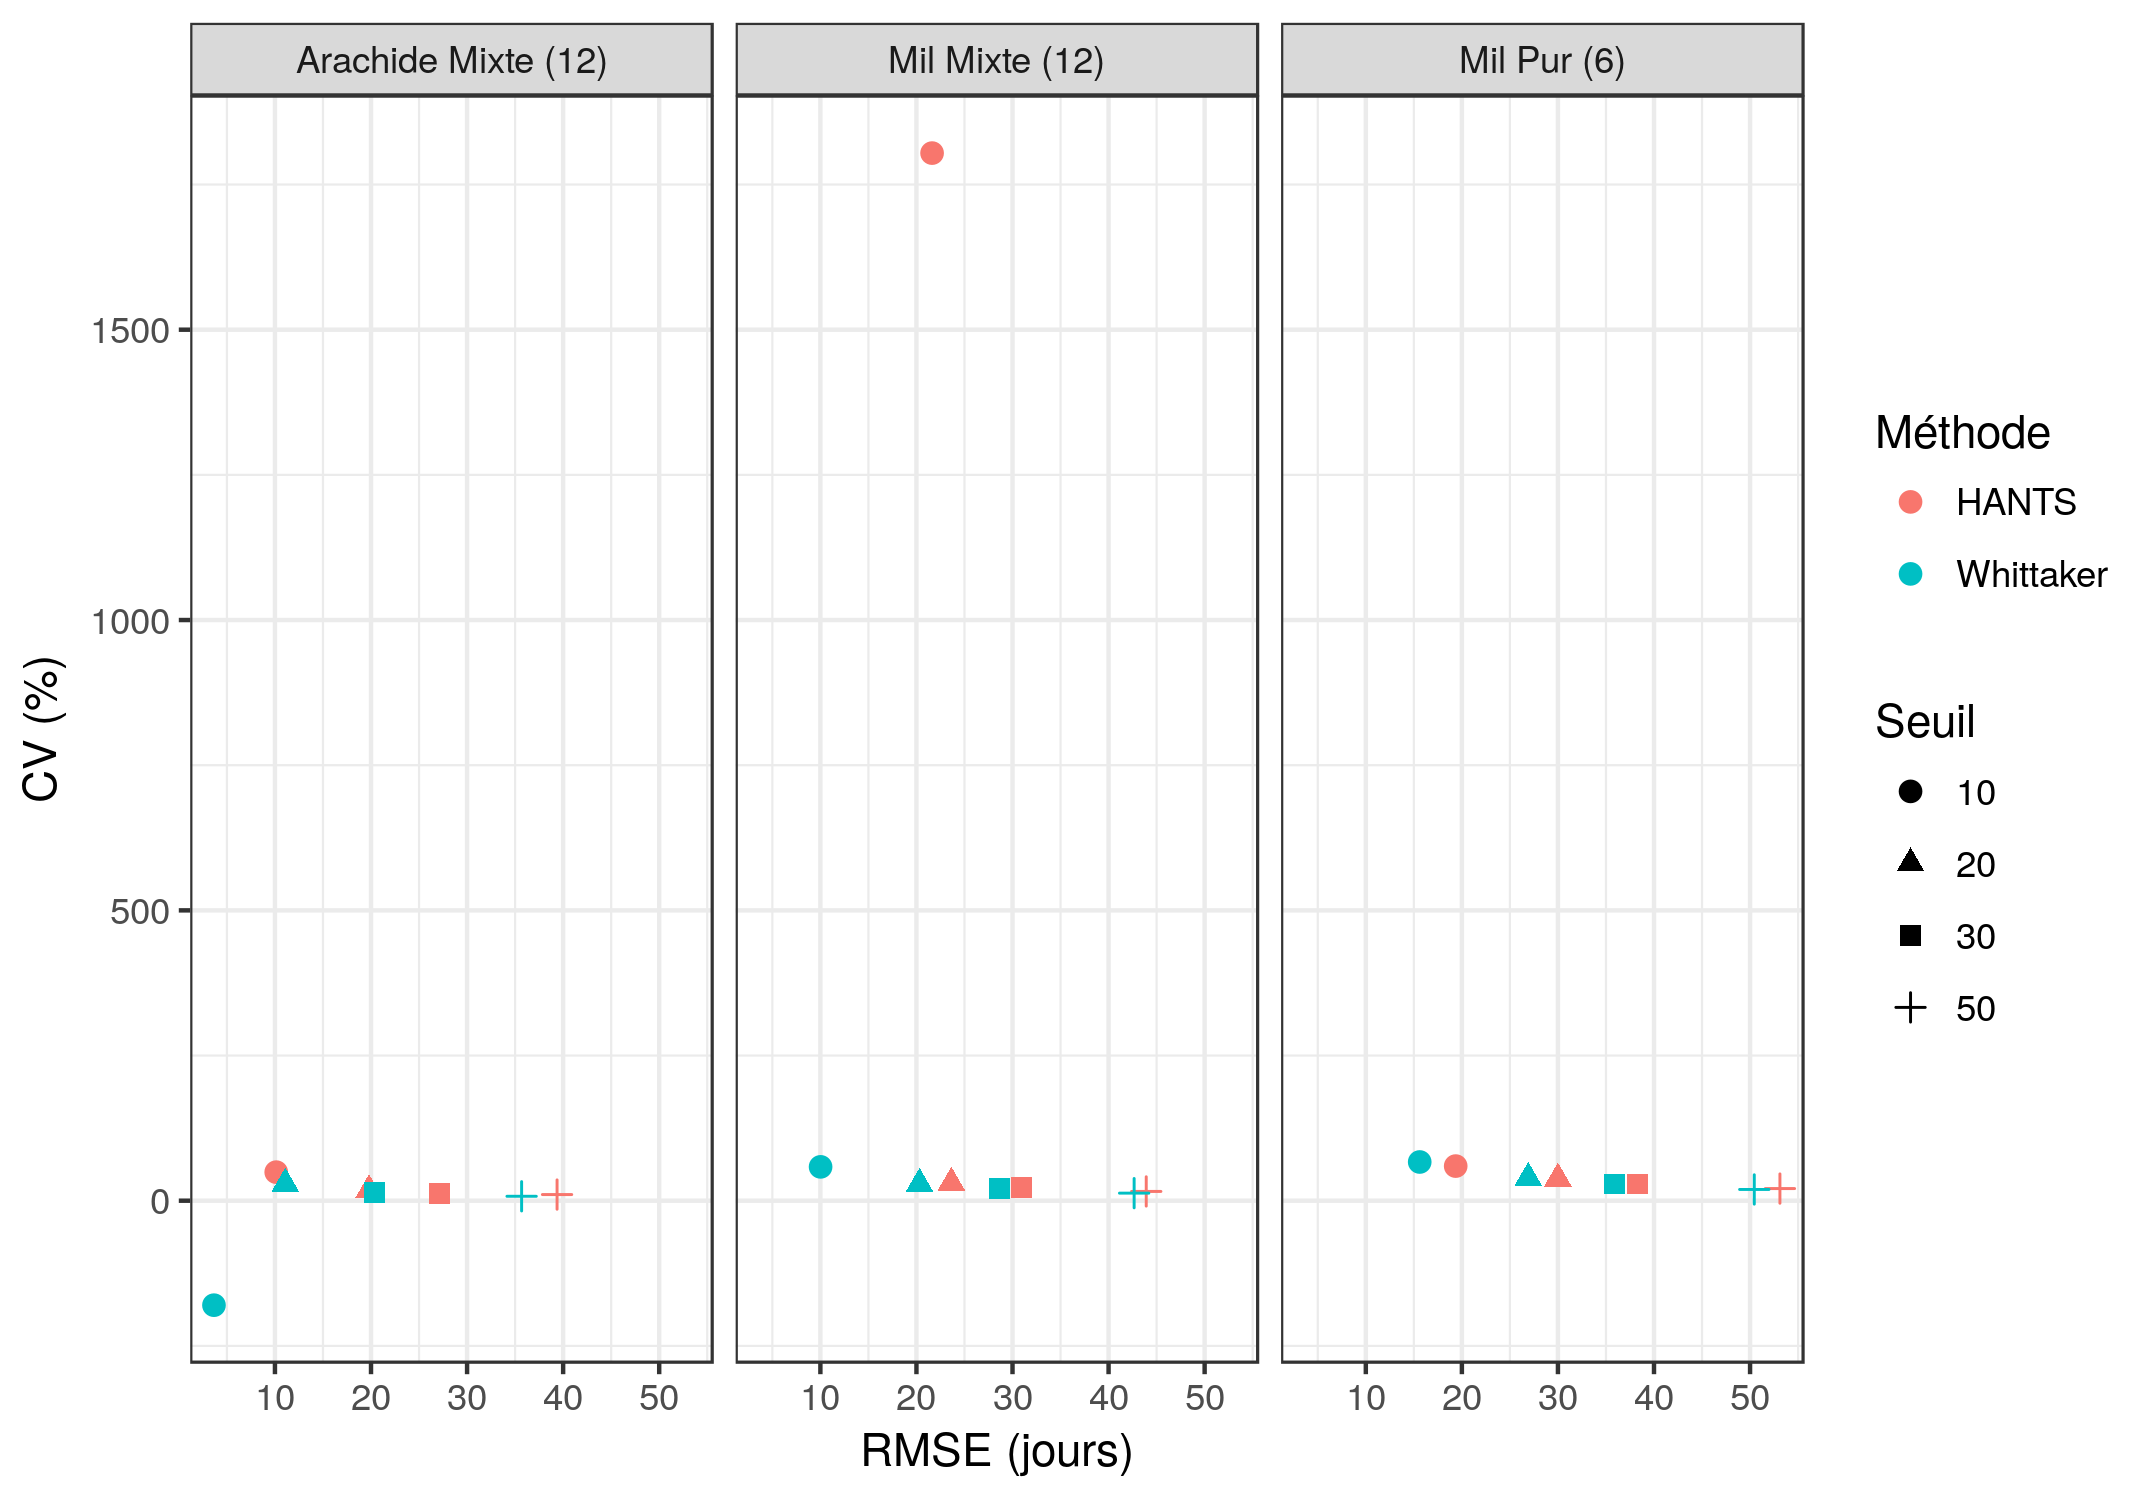
\includegraphics[scale=0.8]{annexes/SOS_RMSE_vs_CV_Oracle.png} 
 \end{center}
 \caption*{SOS : RMSE vs CV}
\end{figure}

\begin{figure}[htbp]
 \begin{center}
  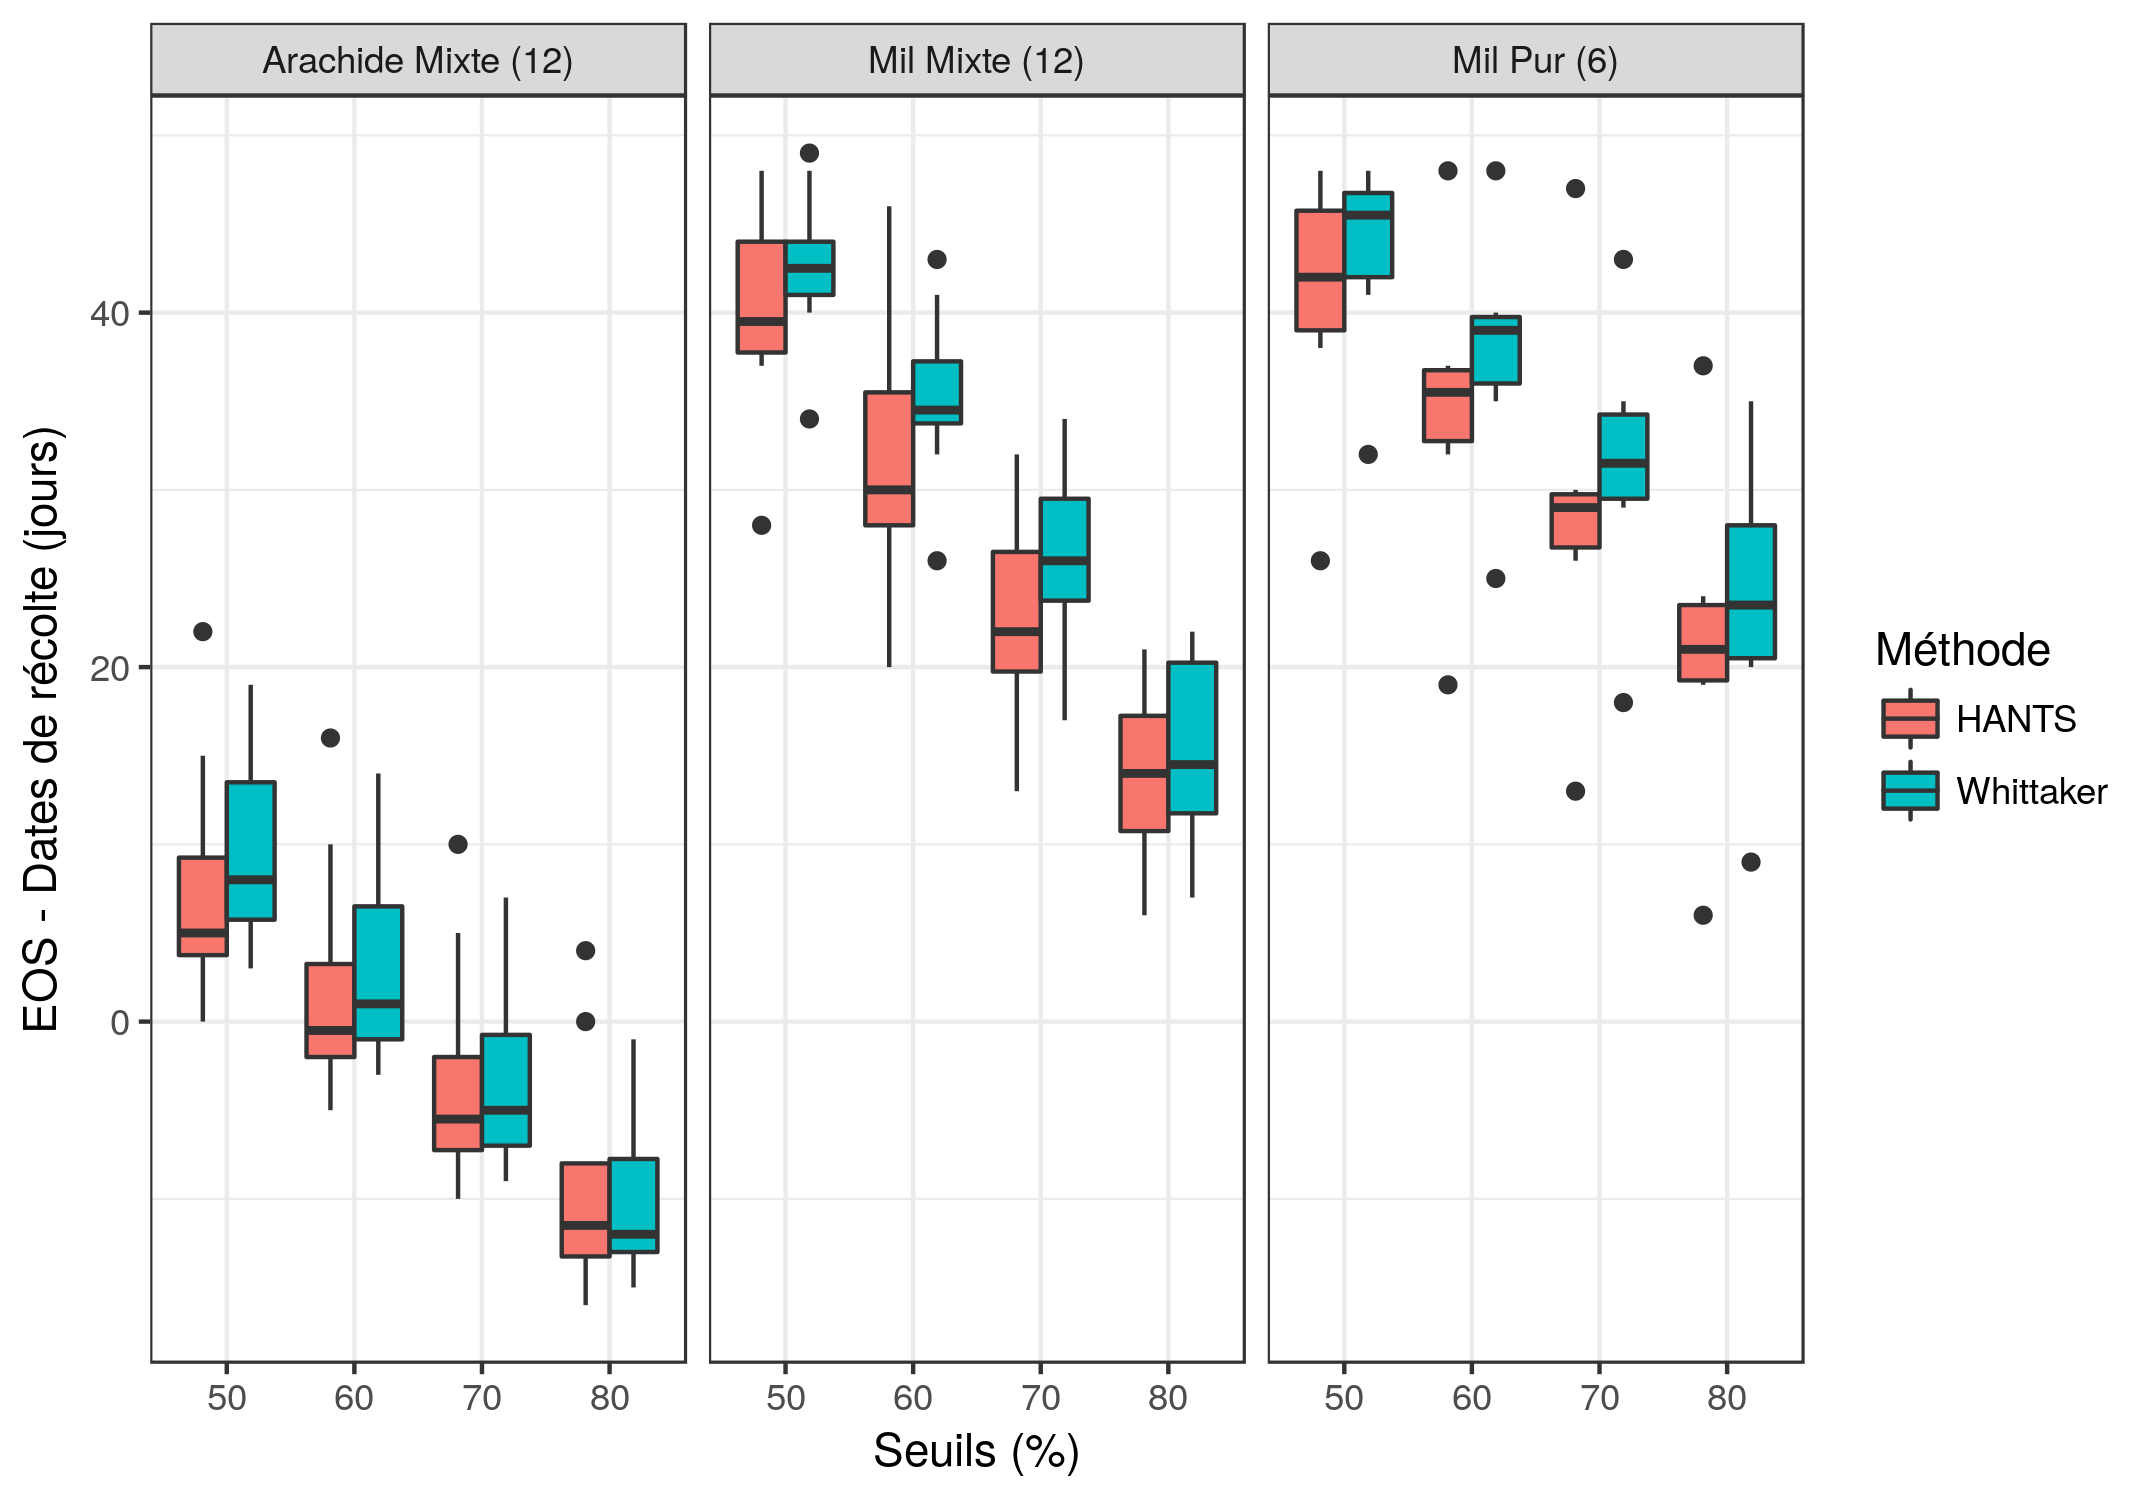
\includegraphics[scale=0.8]{annexes/EOS_Boxplot_Oracle.png} 
 \end{center}
 \caption*{Distribution des écarts entre EOS et dates de récolte}
\end{figure}

\begin{figure}[htbp]
 \begin{center}
  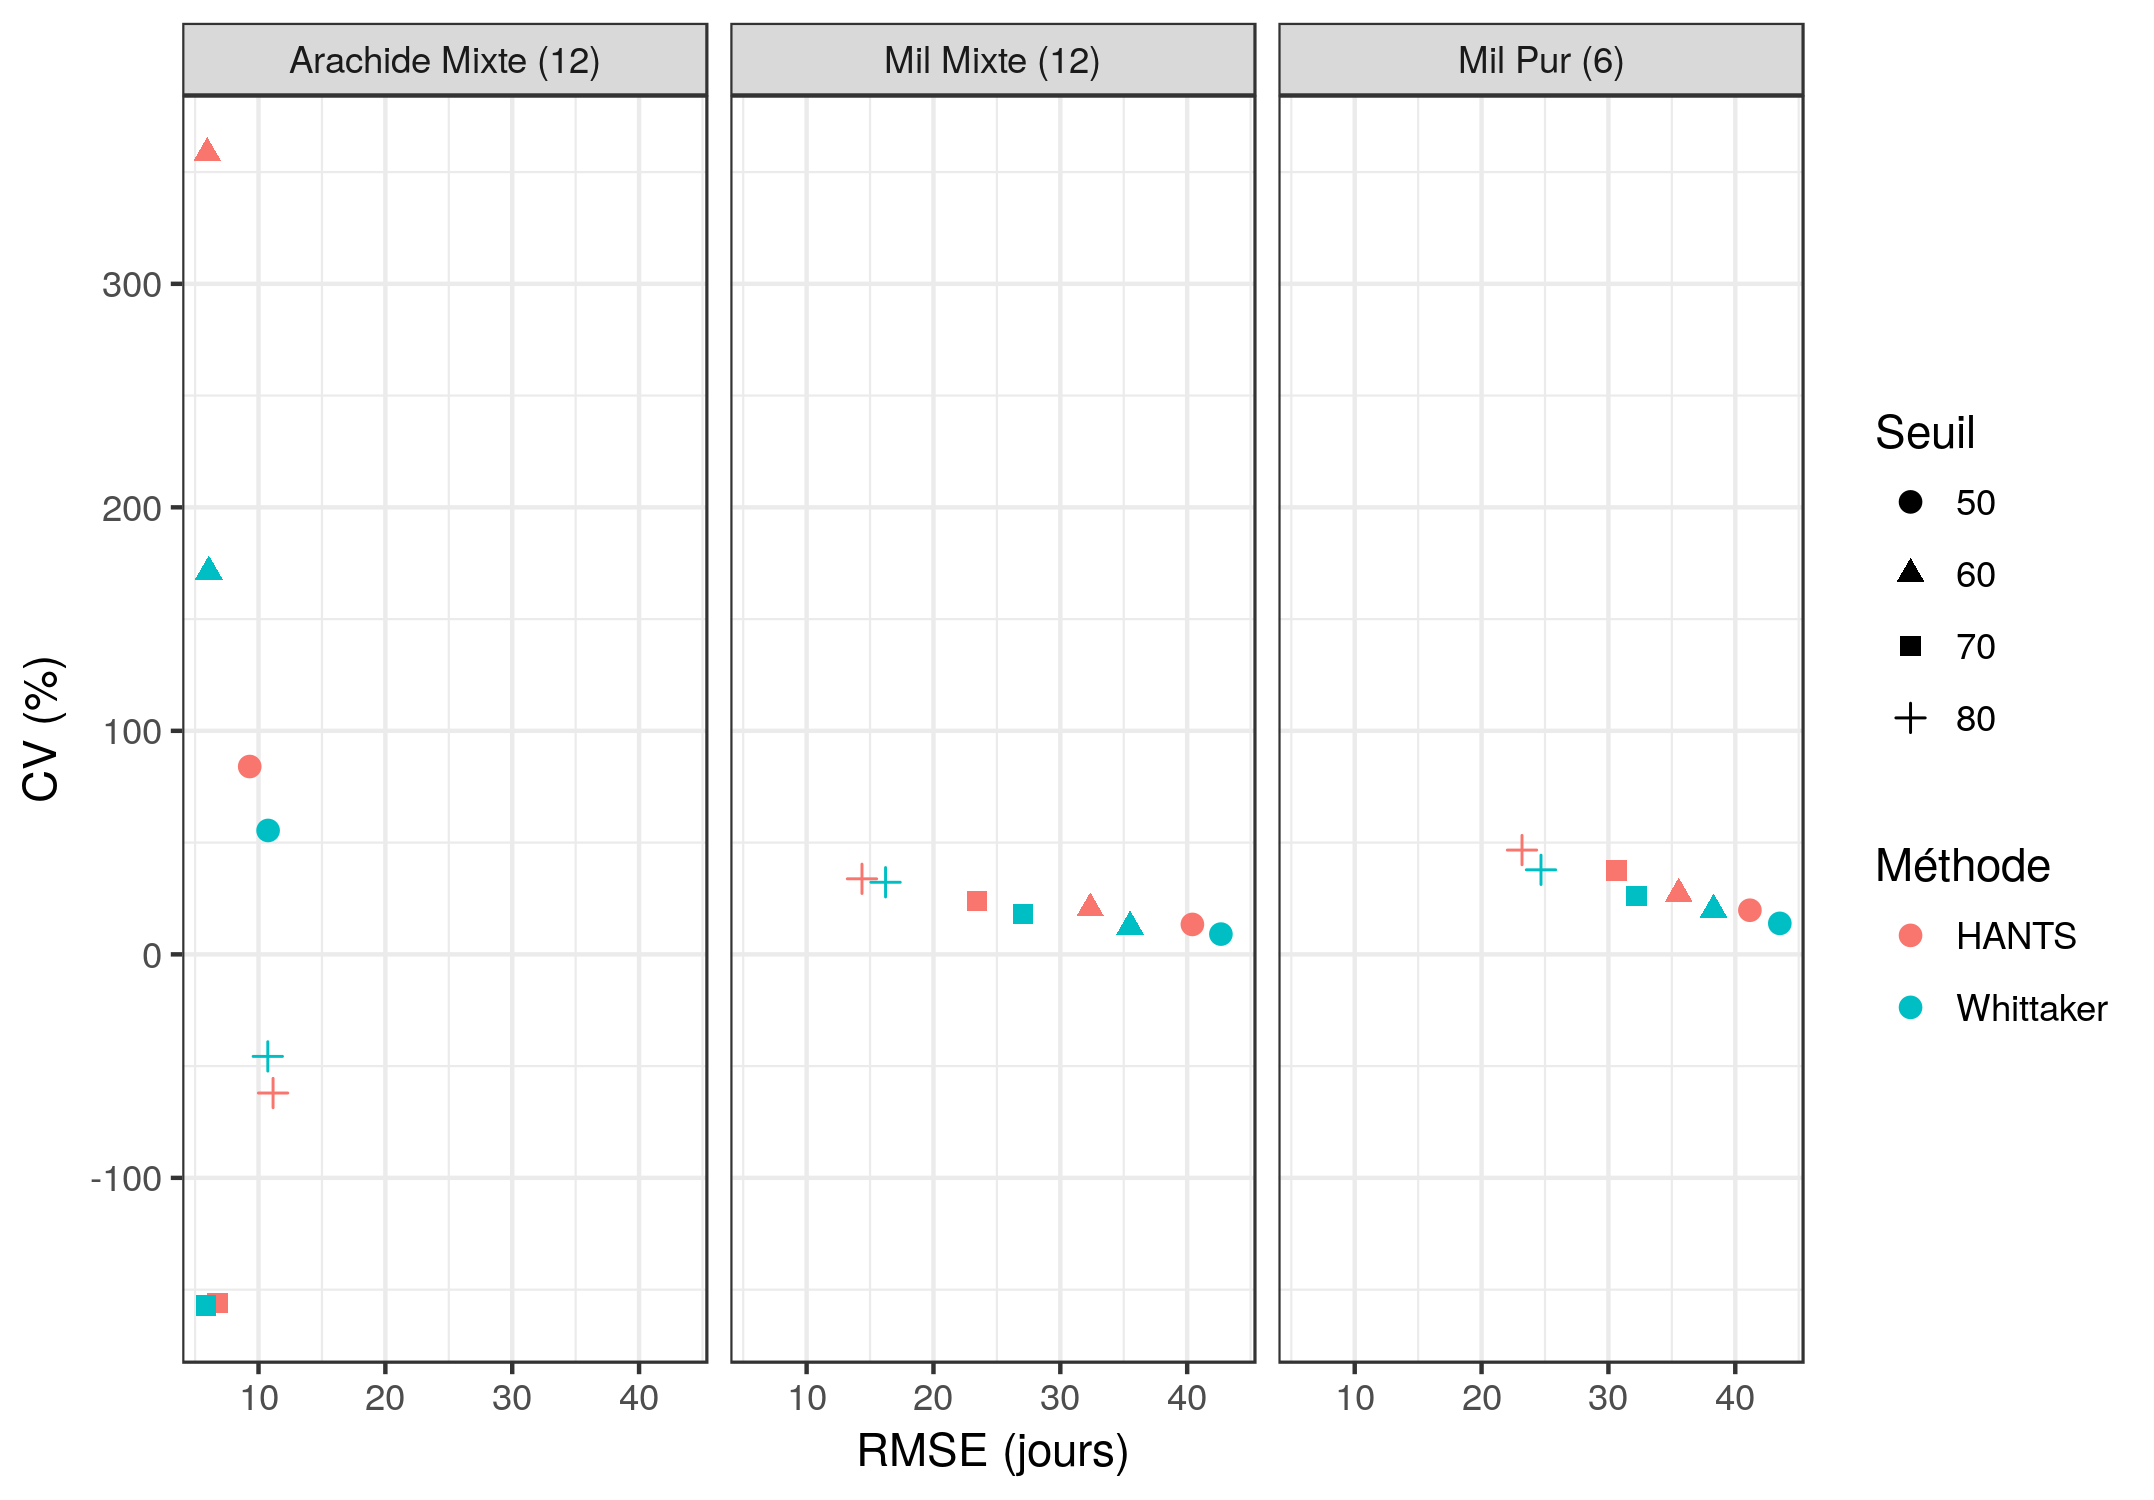
\includegraphics[scale=0.8]{annexes/EOS_RMSE_vs_CV_Oracle.png} 
 \end{center}
 \caption*{EOS : RMSE vs CV}
\end{figure}

\chapter{Spatialisation des SOS et EOS}\label{annexe-d}

La spatialisation des SOS et EOS à l’échelle pixellaire (3 mètres) avec les seuils
adoptés met bien en évidence les zones de jachère sur les cartes produites.

\vspace{8mm}

\begin{figure}[htbp]
 \begin{center}
  \fbox{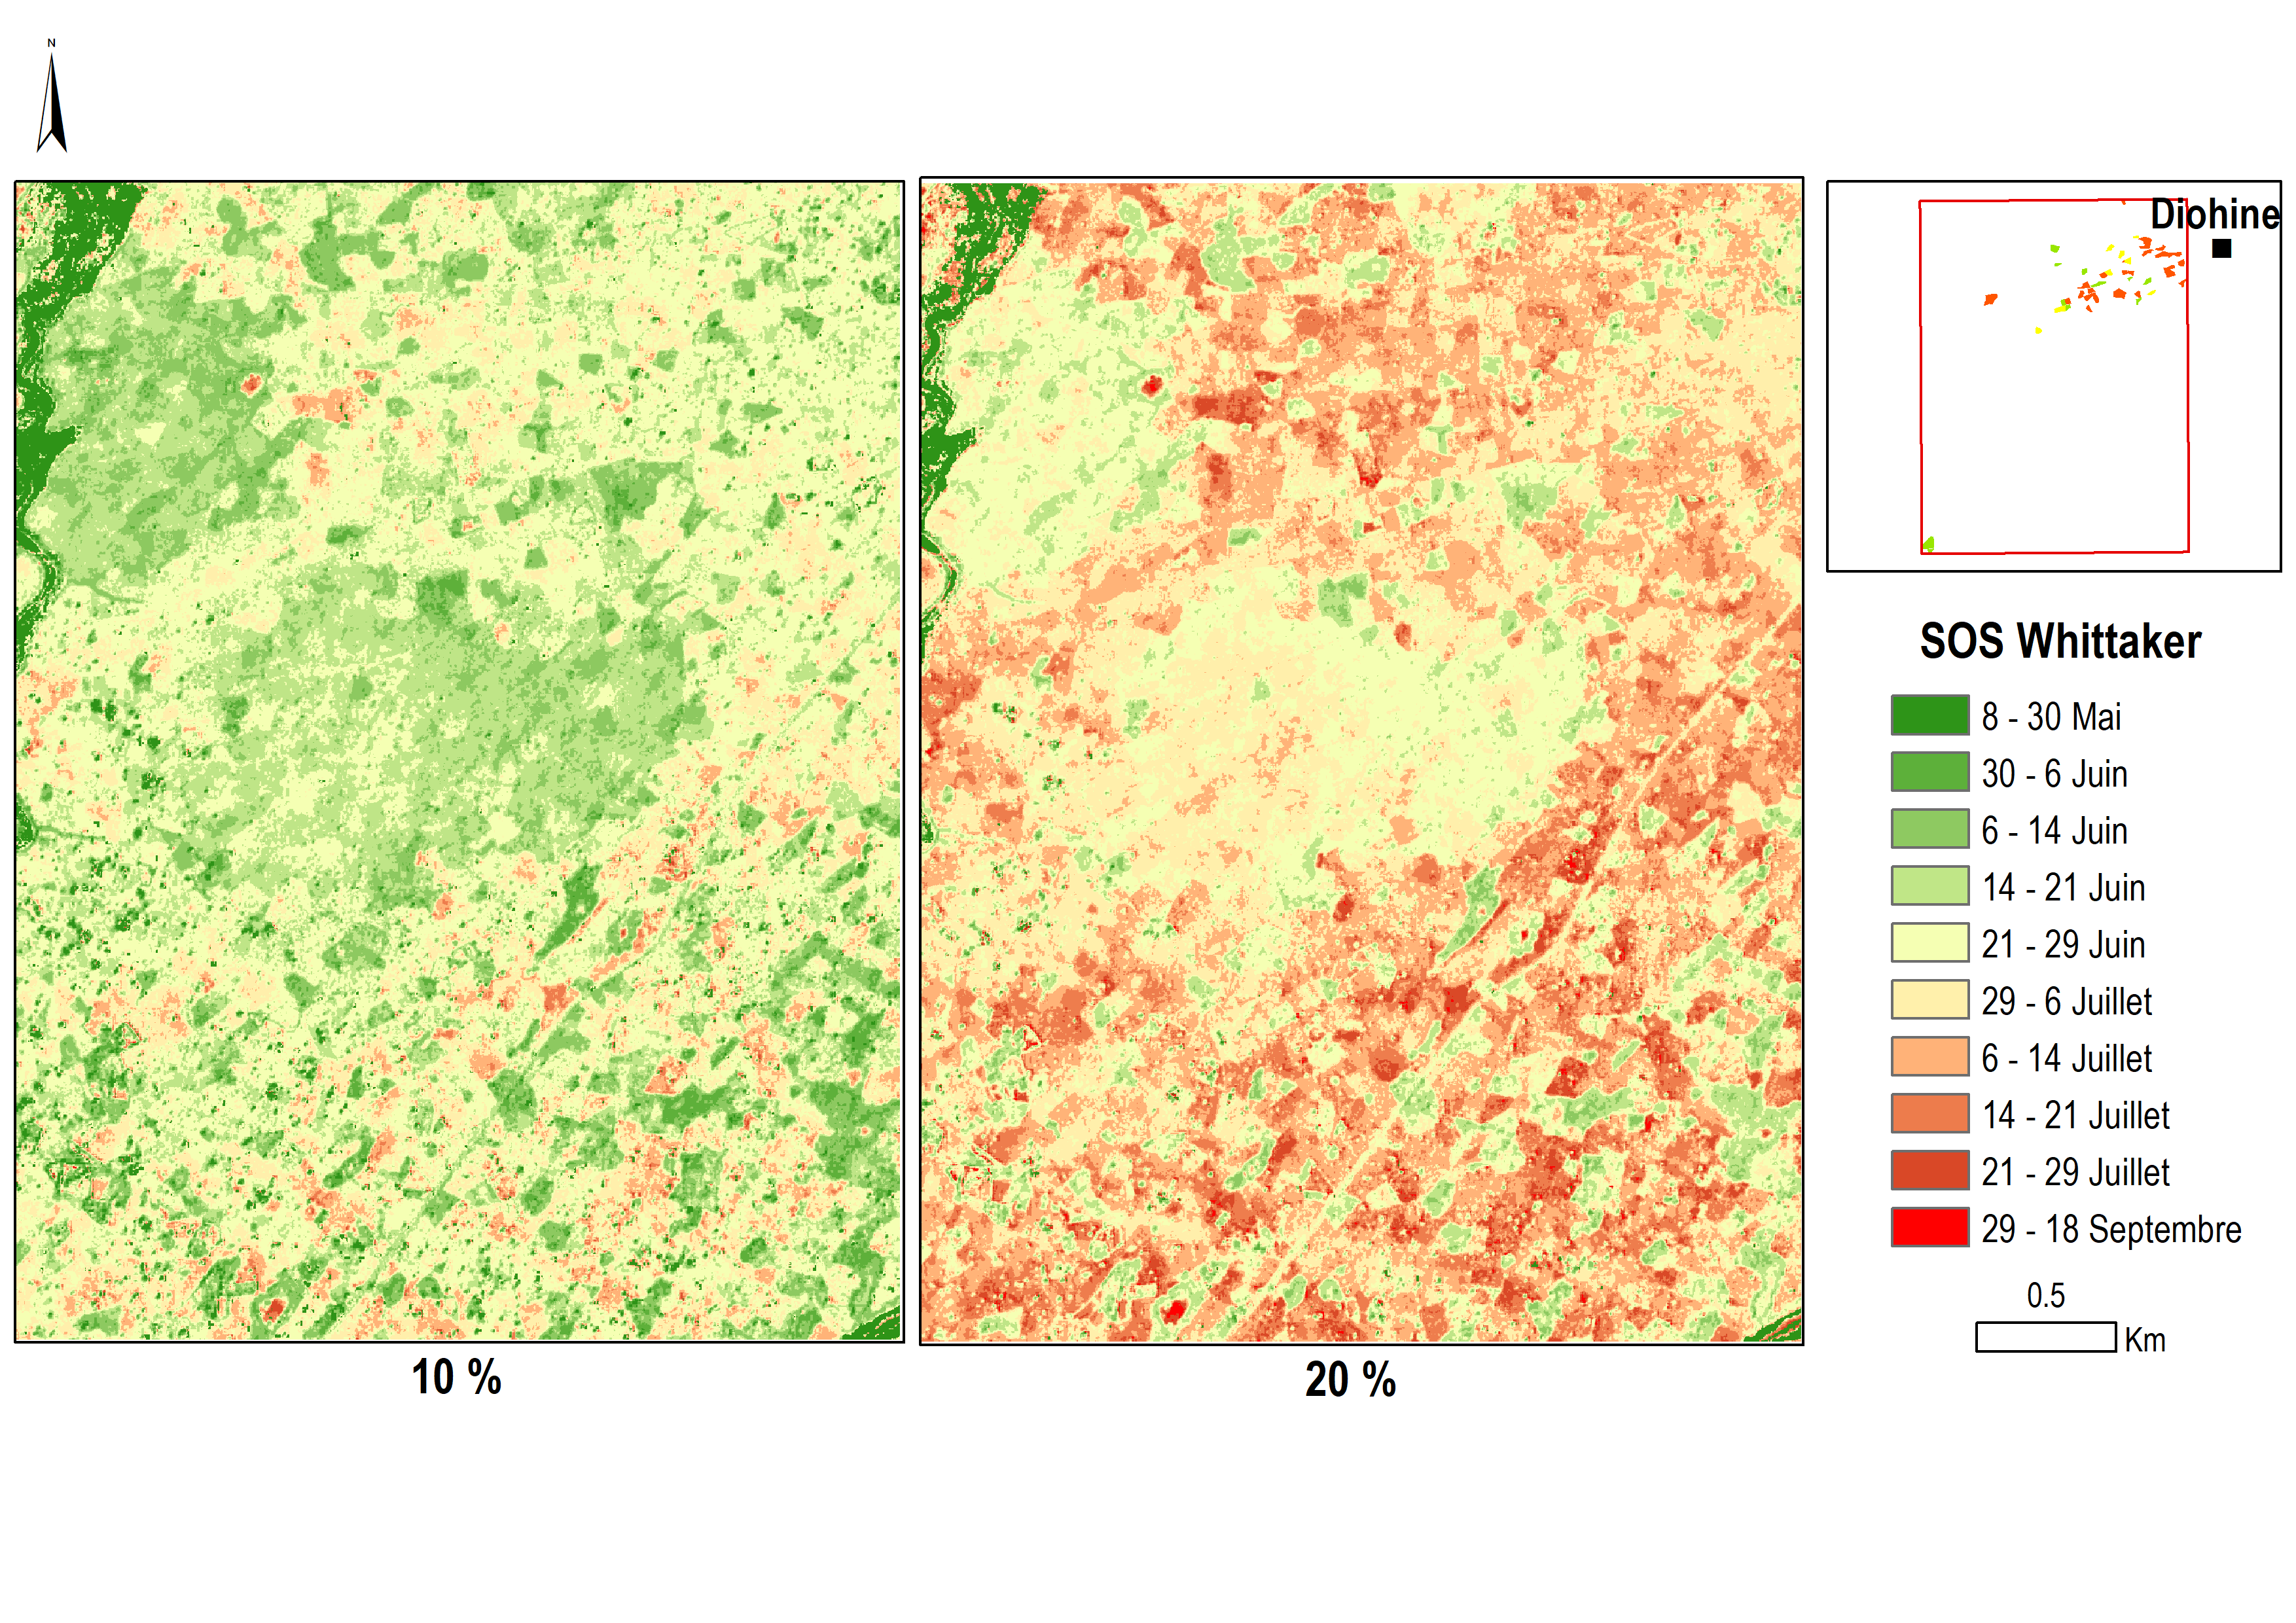
\includegraphics[scale=0.52]{annexes/spatial_sos.png}}
 \end{center}
 \caption*{Spatialisation des SOS}
\end{figure}

\begin{figure}[htbp]
 \begin{center}
  \fbox{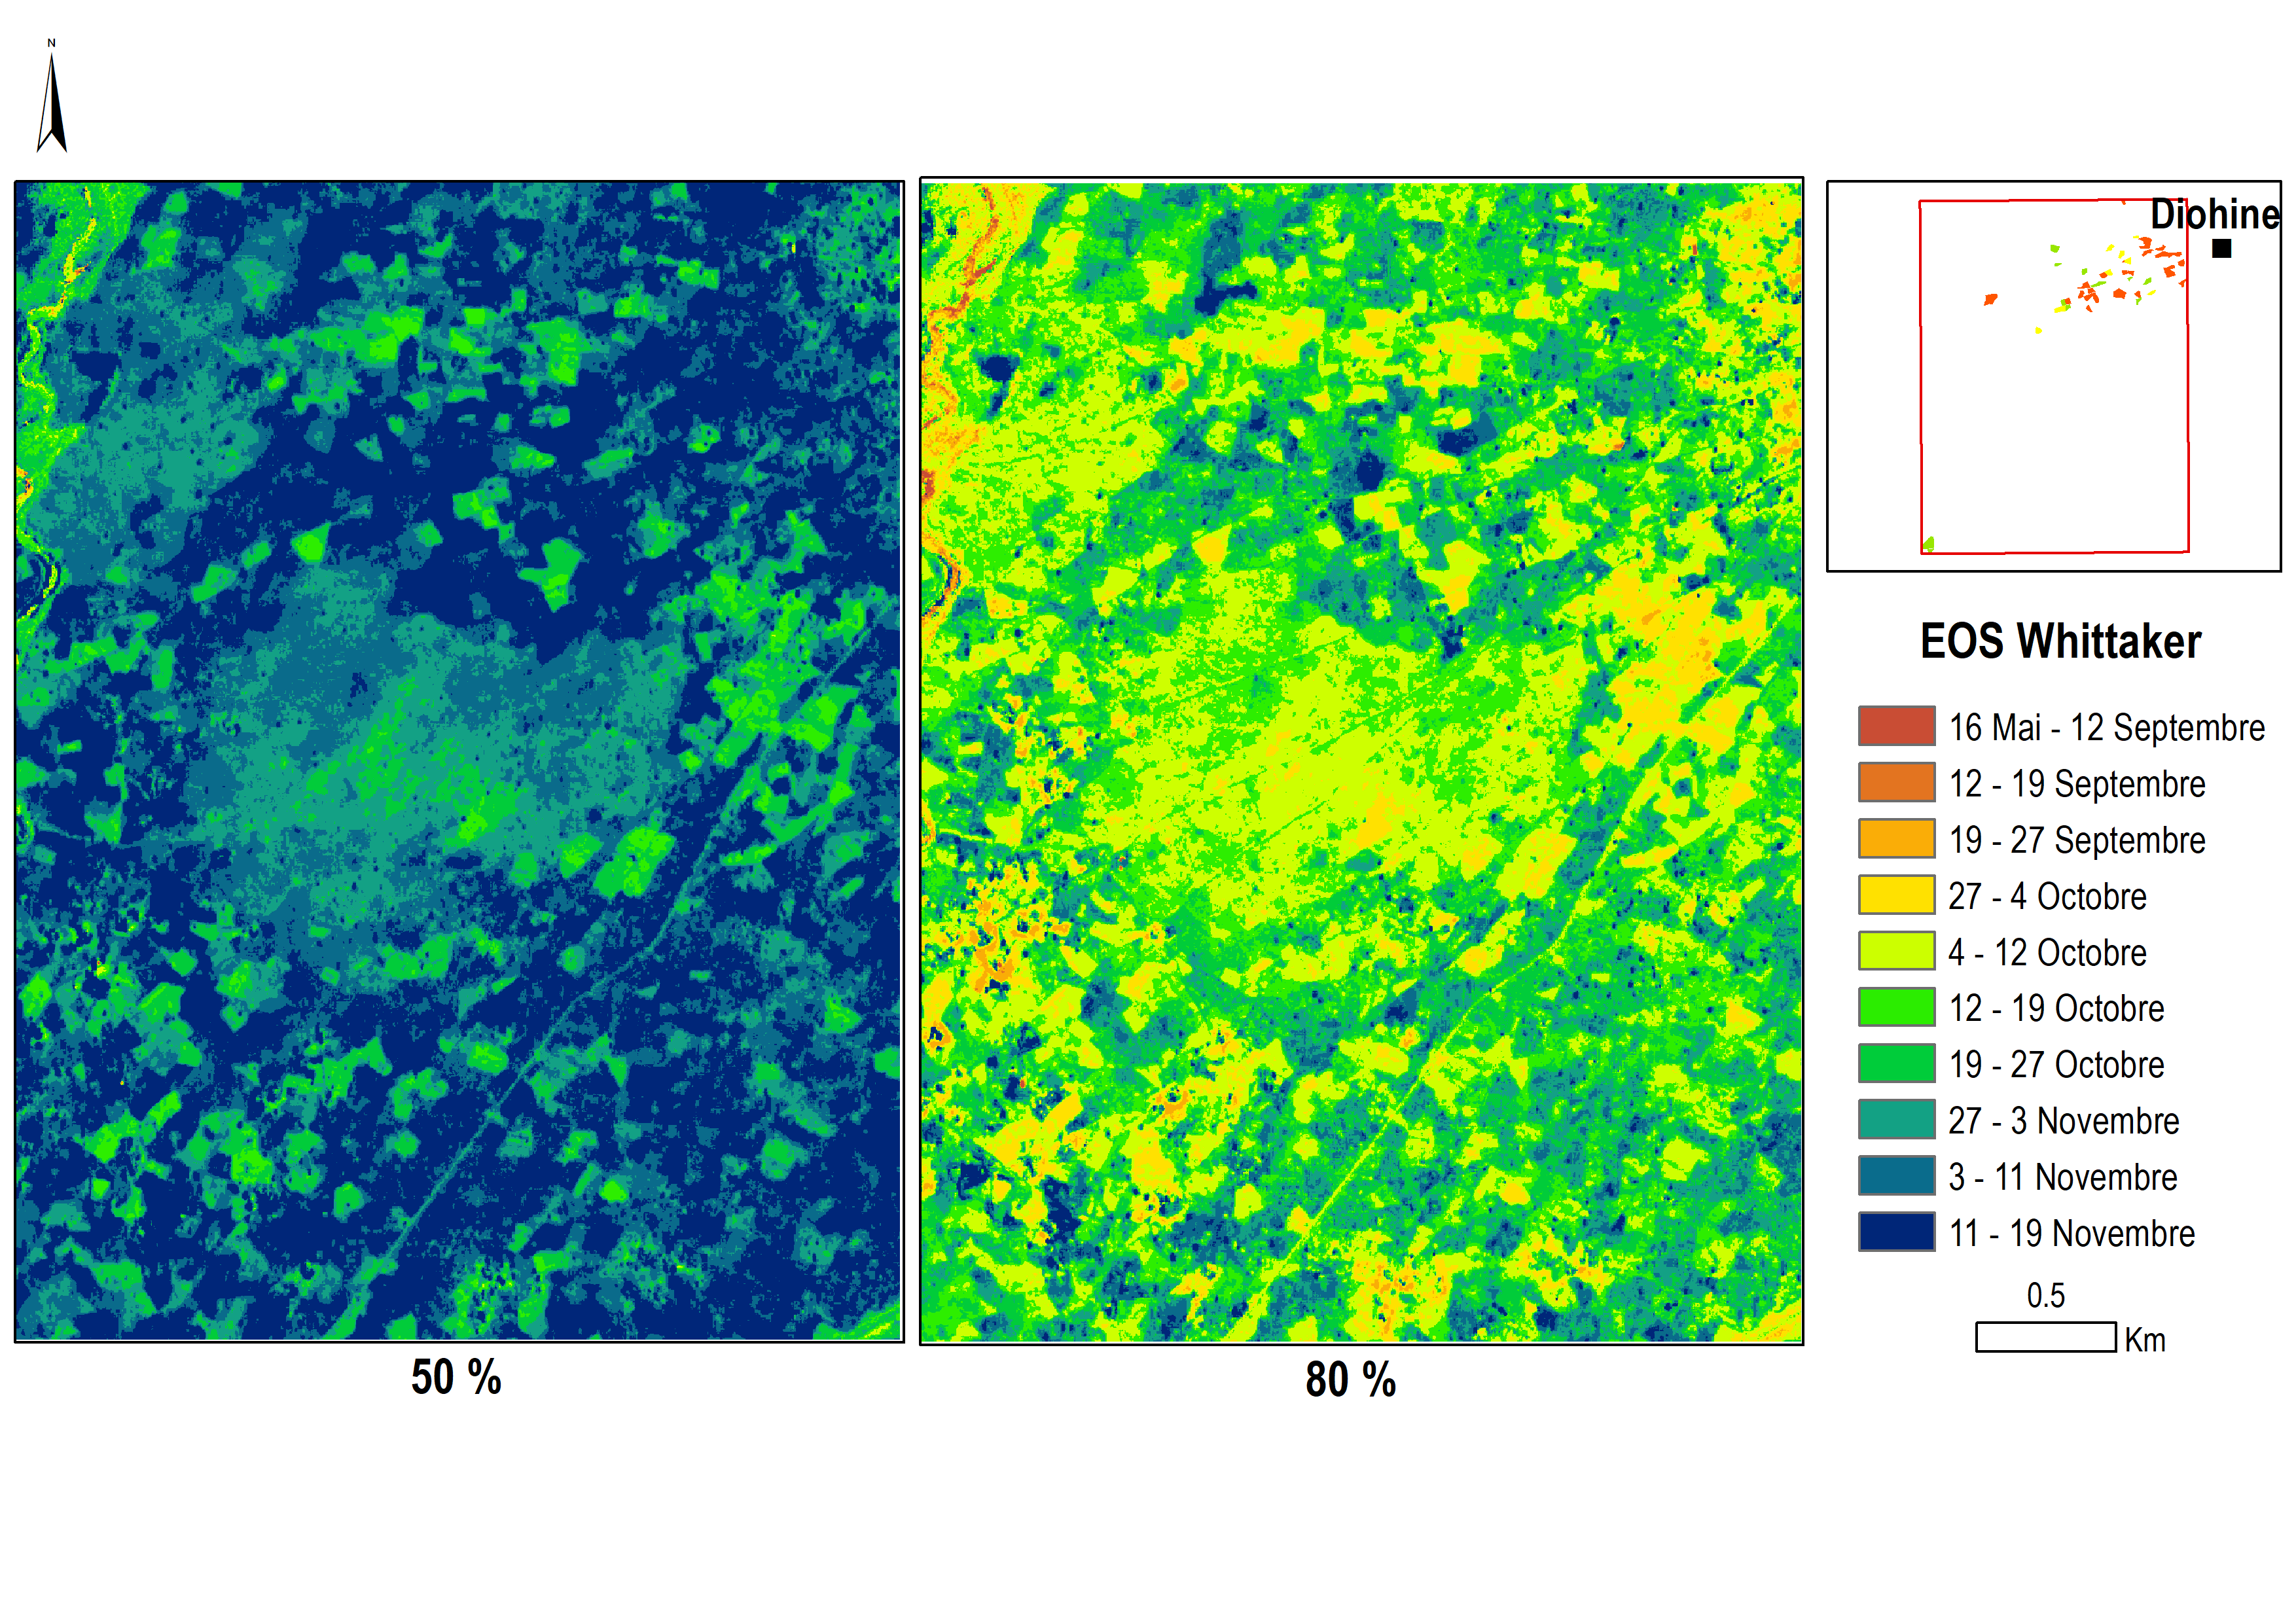
\includegraphics[scale=0.52]{annexes/spatial_eos.png}}
 \end{center}
 \caption*{Spatialisation des EOS}
\end{figure}

\chapter{Relations linéaires entre biomasses et rendements}\label{annexe-e}

\begin{figure}[htbp]
\caption*{Régression linéaire entre la biomasse végétative et le rendement gousse de l’arachide}
 \begin{center}
  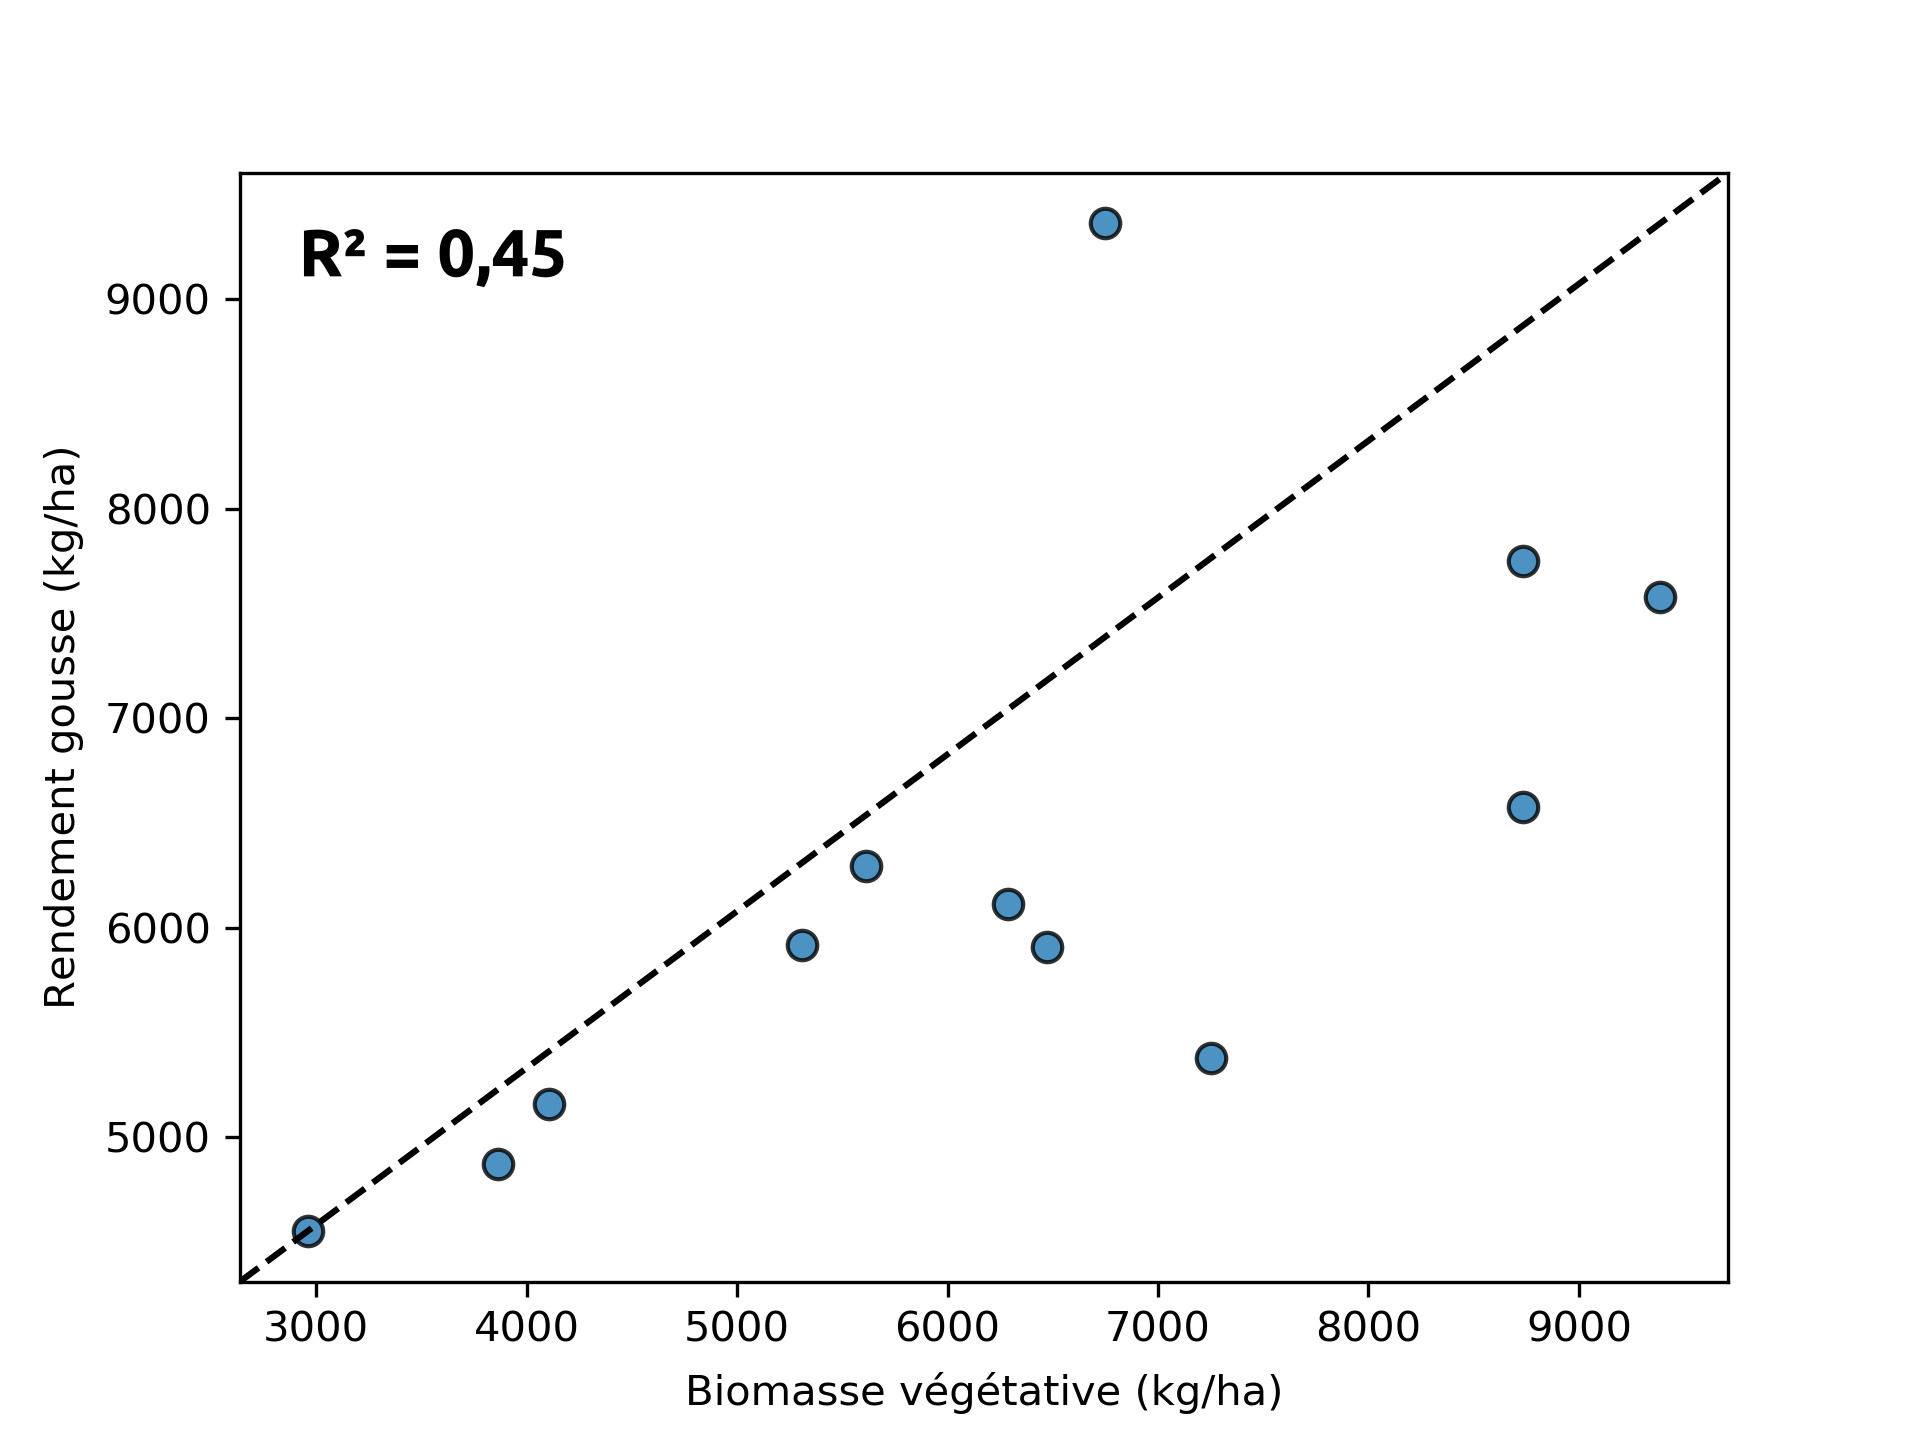
\includegraphics[scale=0.6]{annexes/Biom_vs_Rdt_Arachide.png}
 \end{center}
\end{figure}

\begin{figure}[htbp]
\caption*{Régression linéaire entre la biomasse végétative et le rendement grain du mil}
 \begin{center}
  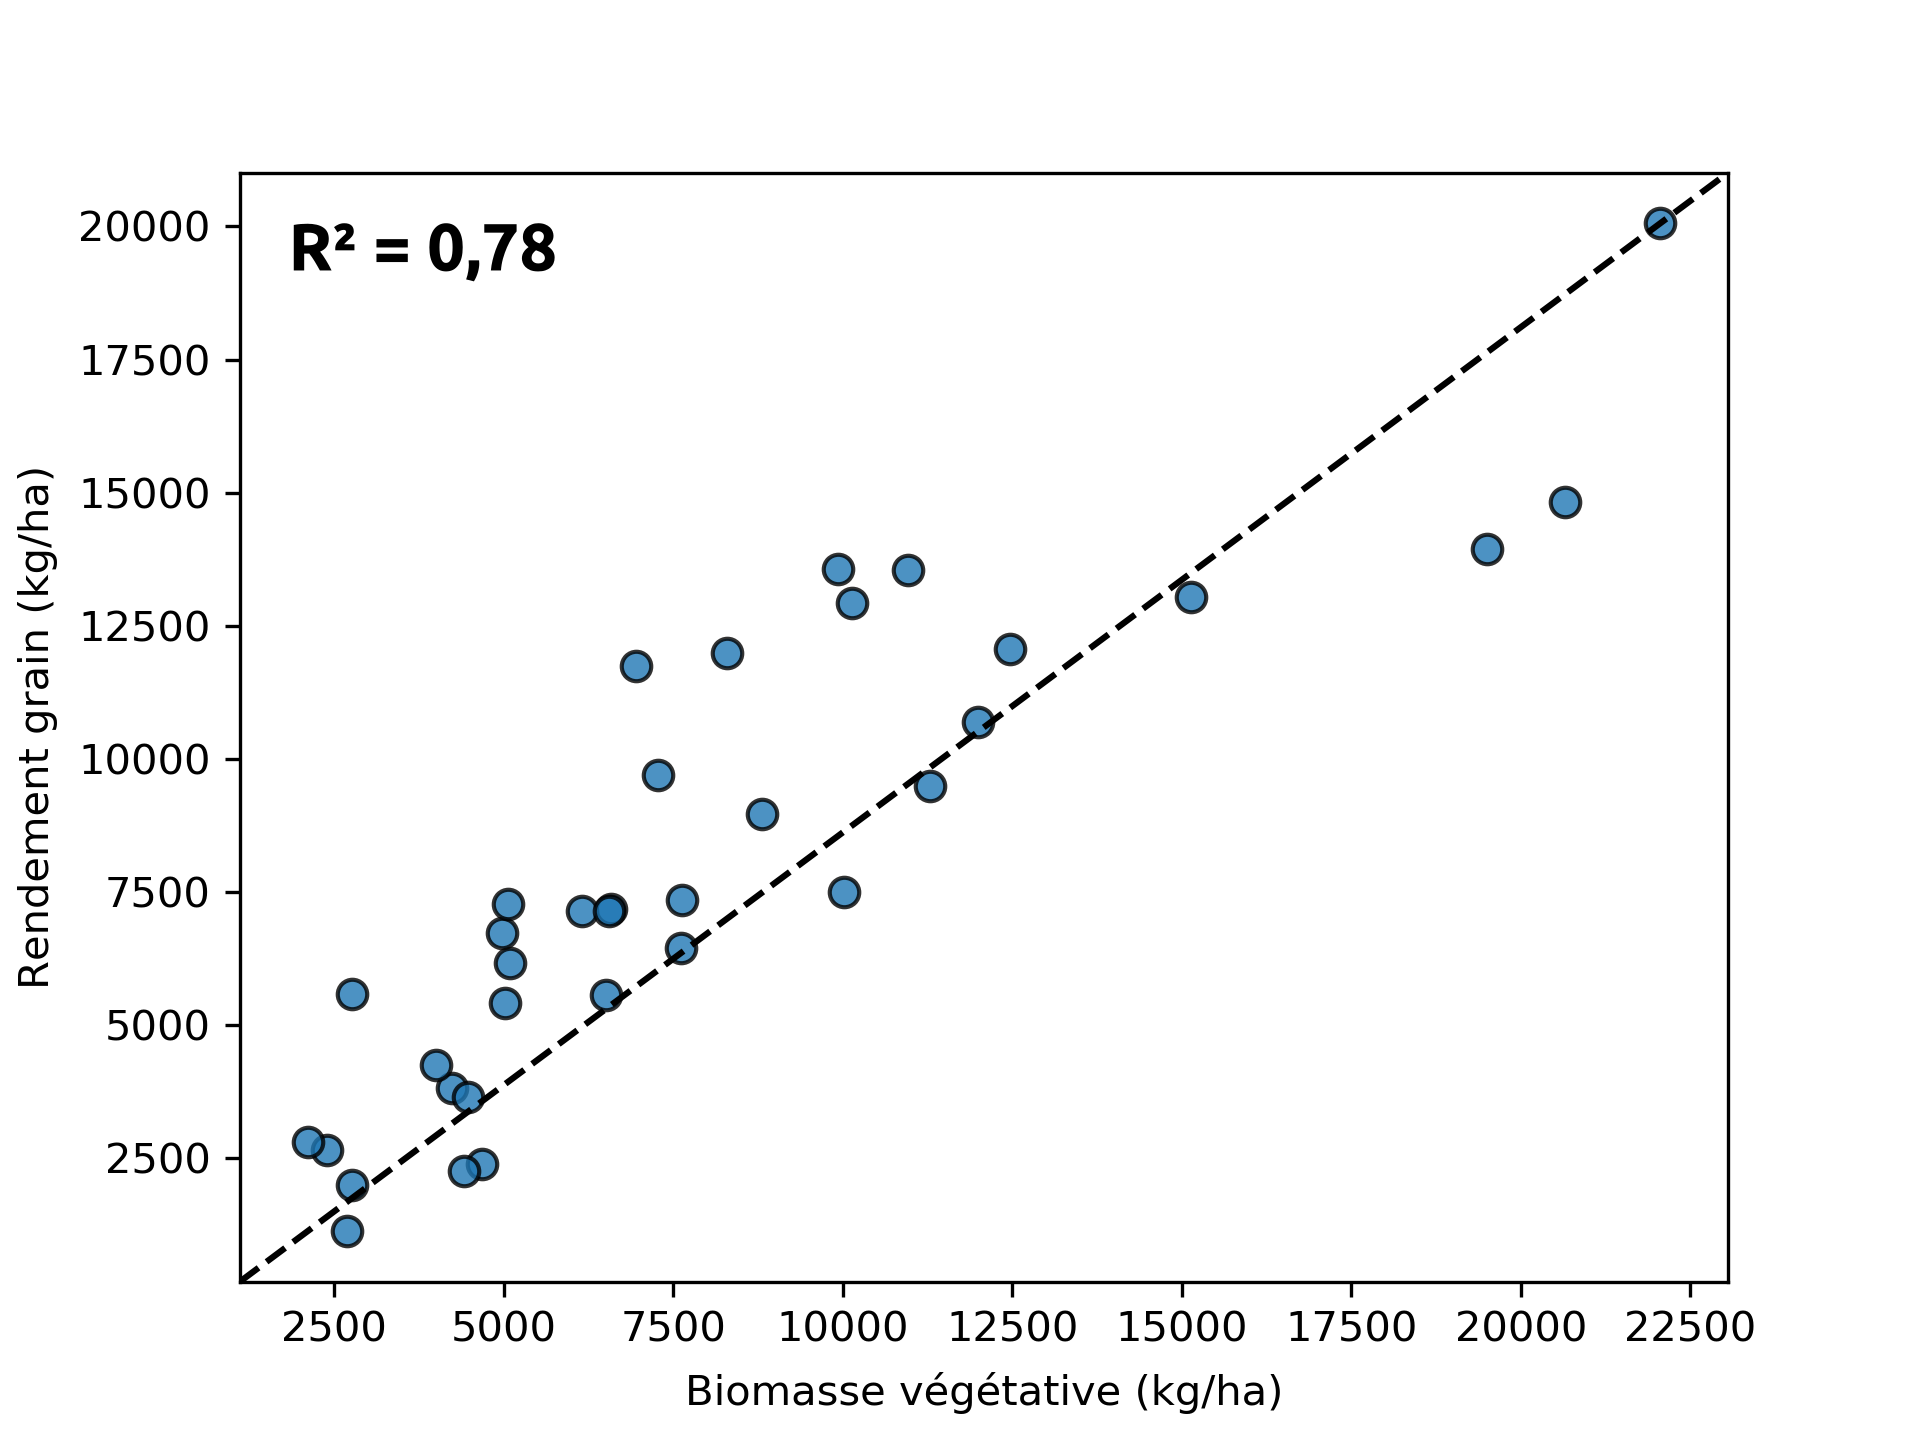
\includegraphics[scale=0.6]{annexes/Biom_vs_Rdt_Mil.png}
 \end{center}
\end{figure}

